% -*- coding: utf-8; -*-

\chapter{Resultados}
\label{ch:result}

	Este capítulo apresenta os resultados desta dissertação para volumes de malhas regulares conhecidos na literatura e modelos de simulação de reservatório de petróleo, respectivamente nas Seções~\ref{sec:result.reg}~e~\ref{sec:result.irreg}. Esses resultados serão comparados com os obtidos através da aplicação do método de \textit{Kindlmann e Durkin}~\cite{gordon}. Para os volumes não regulares, oriundos de simulações de reservatório de petróleo, as derivadas são calculadas de acordo com a Subseção~\ref{subsec:my.nonstruct}.
	
	É preciso lembrar, contudo, que existem diversas técnicas de visualização volumétrica. Então, a análise feita será sempre em cima da função de transferência obtida e como esta foi capaz, ou não, de realçar as fronteiras do volume.
	
	A fim de facilitar a análise dos volumes e suas respectivas funções de transferência geradas pelos dois métodos, utilizou-se uma só escala de cores para todos os volumes, exibida na figura abaixo. O acesso à textura da escala é feito por $ v $, de forma que o primeiro texel é dado por $ v = 0 $ e o último por $ v = 255 $.

\begin{figure}[h]
	\centering
	\includegraphics[width=0.9\textwidth]{images/r_colorscale}
	\caption{Escala de cores das funções de transferência.}
\end{figure}
	
\section{Malhas Regulares}
\label{sec:result.reg}

	Para visualizar os volumes de malhas regulares utilizou-se o visualizador volumétrico apresentado por \textit{Campagnolo et al.}~\cite{lqc}, aplicando o modelo de iluminação de Blinn-Phong e a estratégia \quote{front-to-back composition}, ambos explicados no Capítulo 39 de~\cite{gems}.

%%%%%%%%%%%%%%%%%%%%%%%%%%%%%%%%%% SPHERES %%%%%%%%%%%%%%%%%%%%%%%%%%%%%%%%%%%%%
	A Figura~\ref{fig:r_sphere_slice} exibe uma fatia de um volume sintético com ruido que possui cinco fronteiras próximas aos valores $ 93 $, $ 164 $, $ 178 $, $ 192 $ e $ 210 $. Como pode ser observado na Figura~\ref{fig:r_3sphere}, o método de \textit{Kindlmann e Durkin} identifica duas fronteiras ($ 92 $ e $ 174 $), enquanto o método proposto nesta dissertação identifica quatro ($ 93 $, $ 178 $, $ 203 $ e $ 233 $). A Figura~\ref{fig:r_3sphere}~\ref{fig:r_3sphere_kd} mostra ainda que há dois pontos de máximo local na primeira derivada média (em azul) que não são realçados como fronteira, pois a segunda derivada média nesses pontos não é próxima de zero. Estes mesmos dois picos, descartados pelo método de \textit{Kindlmann e Durkin} coincidem exatamente com as duas fronteiras destacadas a mais pelo método aqui proposto, como mostra a Figura~\ref{fig:r_3sphere}~\ref{fig:r_3sphere_mine}.
	
\begin{figure}[h]
	\centering
	\includegraphics[width=0.47\textwidth]{images/r_3sphere_slice}
	\caption{Fatia do volume \quote{Test Spheres}.}
	\label{fig:r_sphere_slice}
\end{figure}

\begin{figure}[h]
	\centering
	\subfigure[Método de \textit{Kindlmann e Durkin}.]
	{
		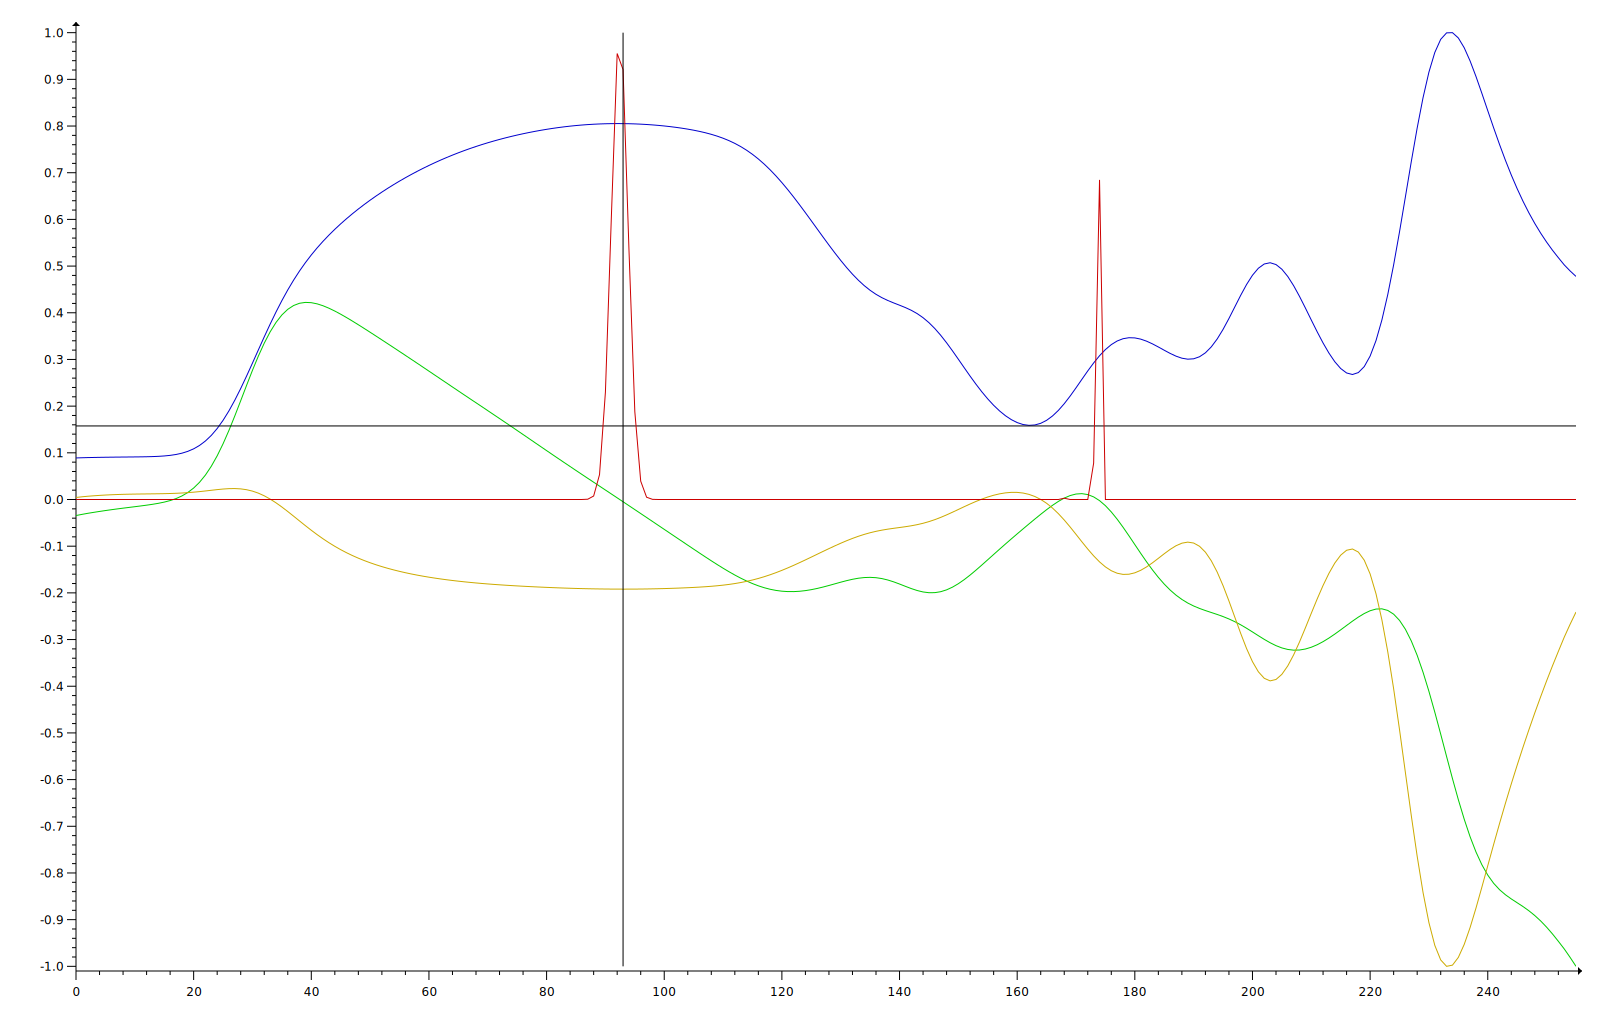
\includegraphics[width=0.35\textwidth]{images/r_g_3sphere}
		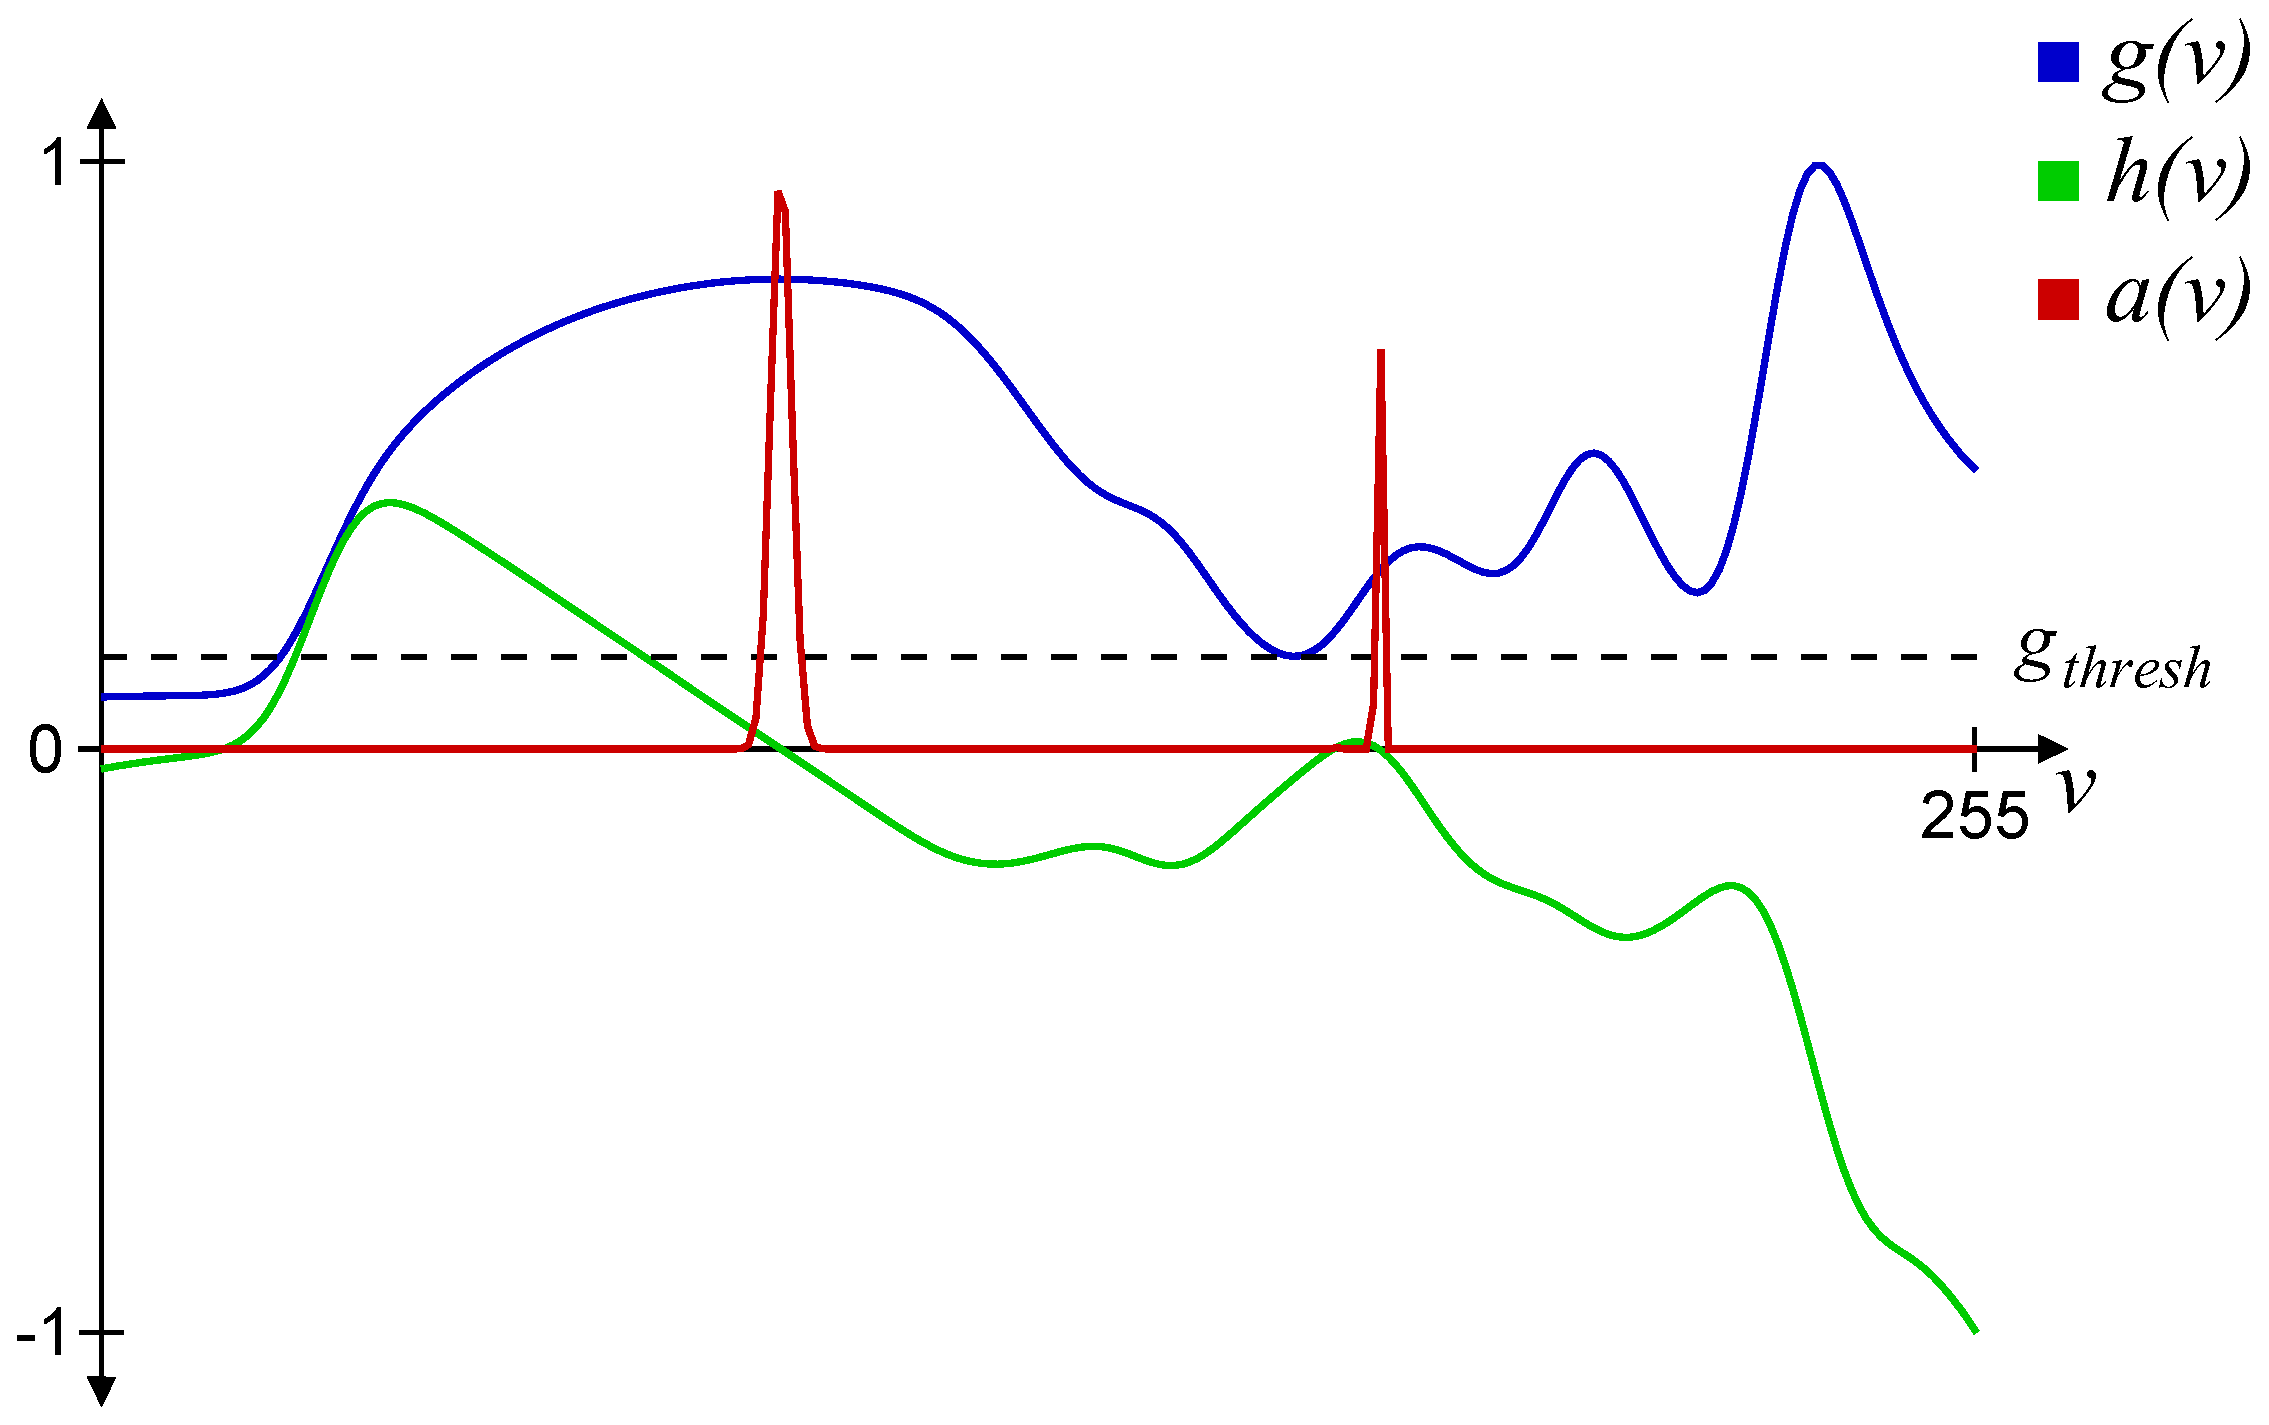
\includegraphics[width=0.65\textwidth]{images/r_g_3sphere_ft}
		\label{fig:r_3sphere_kd}
	}
	\subfigure[Método proposto.]
	{
		\includegraphics[width=0.35\textwidth]{images/r_m_3sphere}
		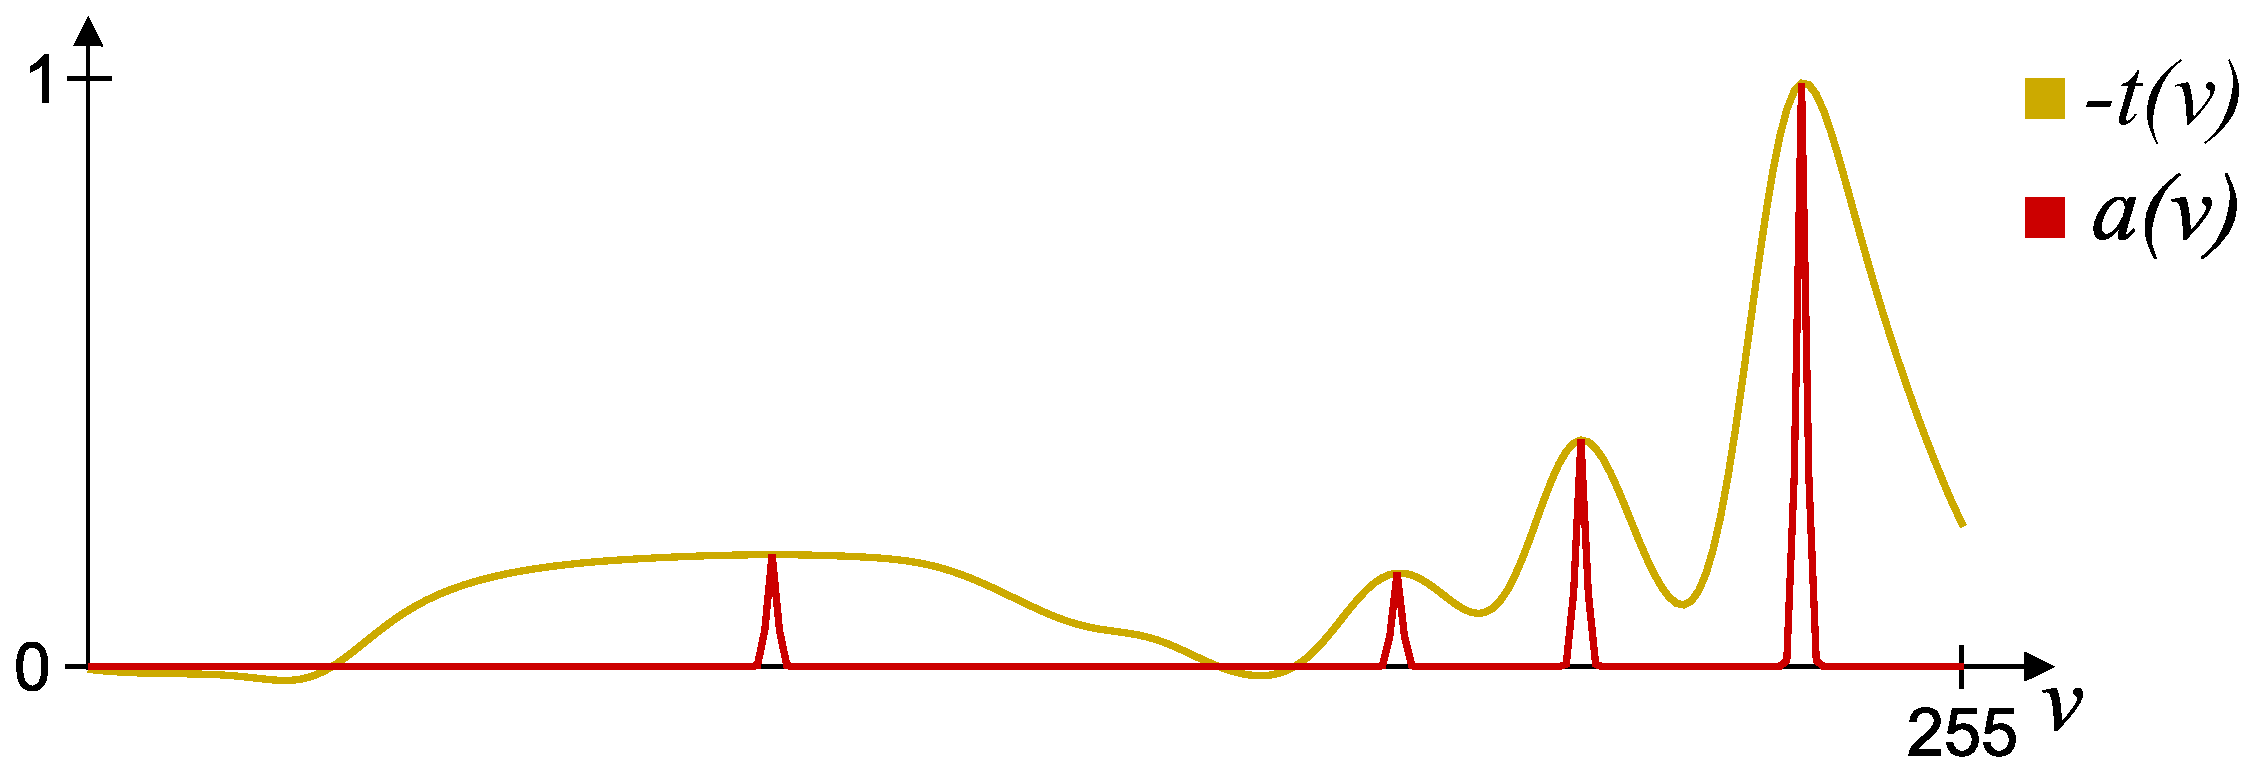
\includegraphics[width=0.65\textwidth]{images/r_m_3sphere_ft}			\label{fig:r_3sphere_mine}
	}
	\caption{Visualização e função de transferência do volume \quote{Test Spheres}.}
	\label{fig:r_3sphere}
\end{figure}

%%%%%%%%%%%%%%%%%%%%%%%%%%%%%%%%%% NUCLEON %%%%%%%%%%%%%%%%%%%%%%%%%%%%%%%%%%%%%
	A Figura~\ref{fig:r_nucleon_slice} mostra uma fatia do volume \quote{Nucleon}. Nela é possível observar duas fronteiras: preto-cinza, cinza-branco. A Figura~\ref{fig:r_nucleon}~\ref{fig:r_nucleon_kd} mostra que o método de \textit{Kindlmann e Durkin} identifica apenas uma fronteira, enquanto o método proposto por esta dissertação identifica as duas existentes, como mostra a Figura~\ref{fig:r_nucleon}~\ref{fig:r_nucleon_mine}. Contudo, ao comparar a fatia do volume com as visualizações, observa-se que a isosuperfície esférica central é mais fielmente representada pela fronteira destacada pelo método de \textit{Kindlmann e Durkin}.
	
\begin{figure}[h]
	\centering
	\includegraphics[width=0.33\textwidth]{images/g_nucleon_slice}
	\caption{Fatia do volume \quote{Nucleon}.}
	\label{fig:r_nucleon_slice}
\end{figure}

\begin{figure}[h]
	\centering
	\subfigure[Método de \textit{Kindlmann e Durkin}.]
	{
		\includegraphics[width=0.3\textwidth]{images/g_nucleon}
		\includegraphics[width=0.65\textwidth]{images/r_g_nucleon_ft}
		\label{fig:r_nucleon_kd}
	}
	\subfigure[Método proposto.]
	{
		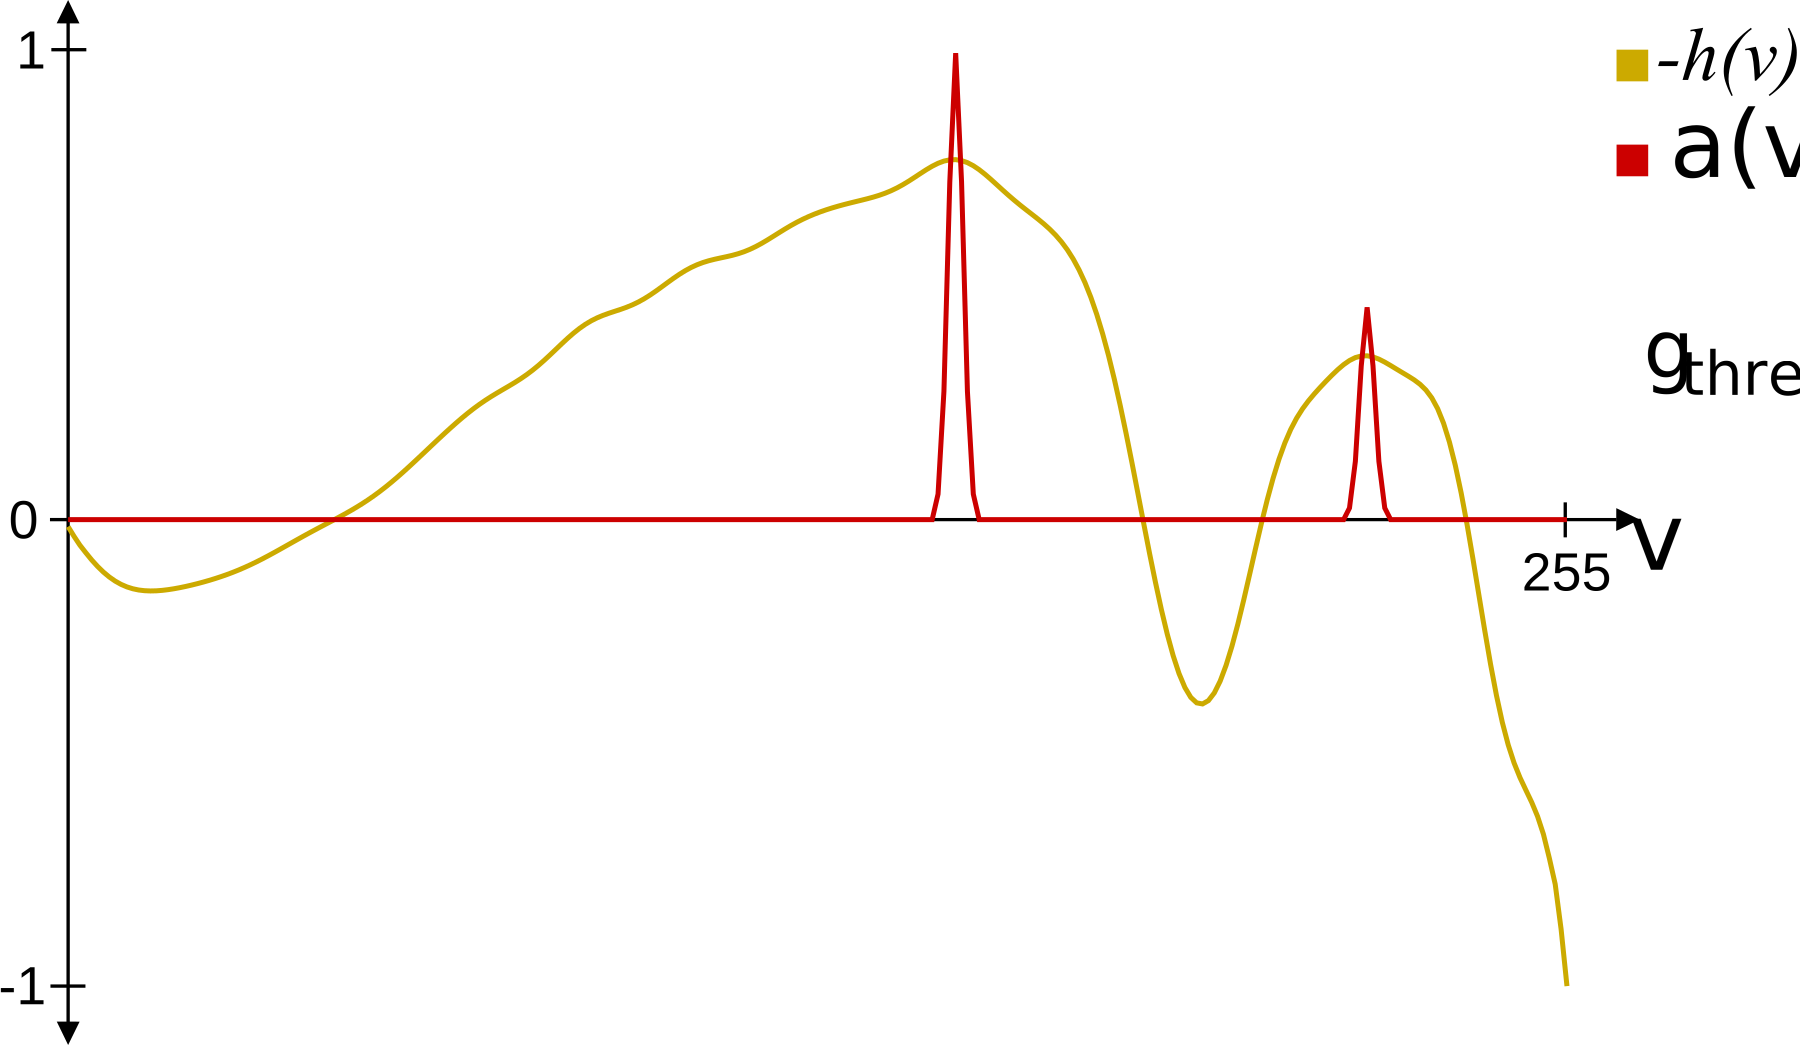
\includegraphics[width=0.3\textwidth]{images/r_m_nucleon}
		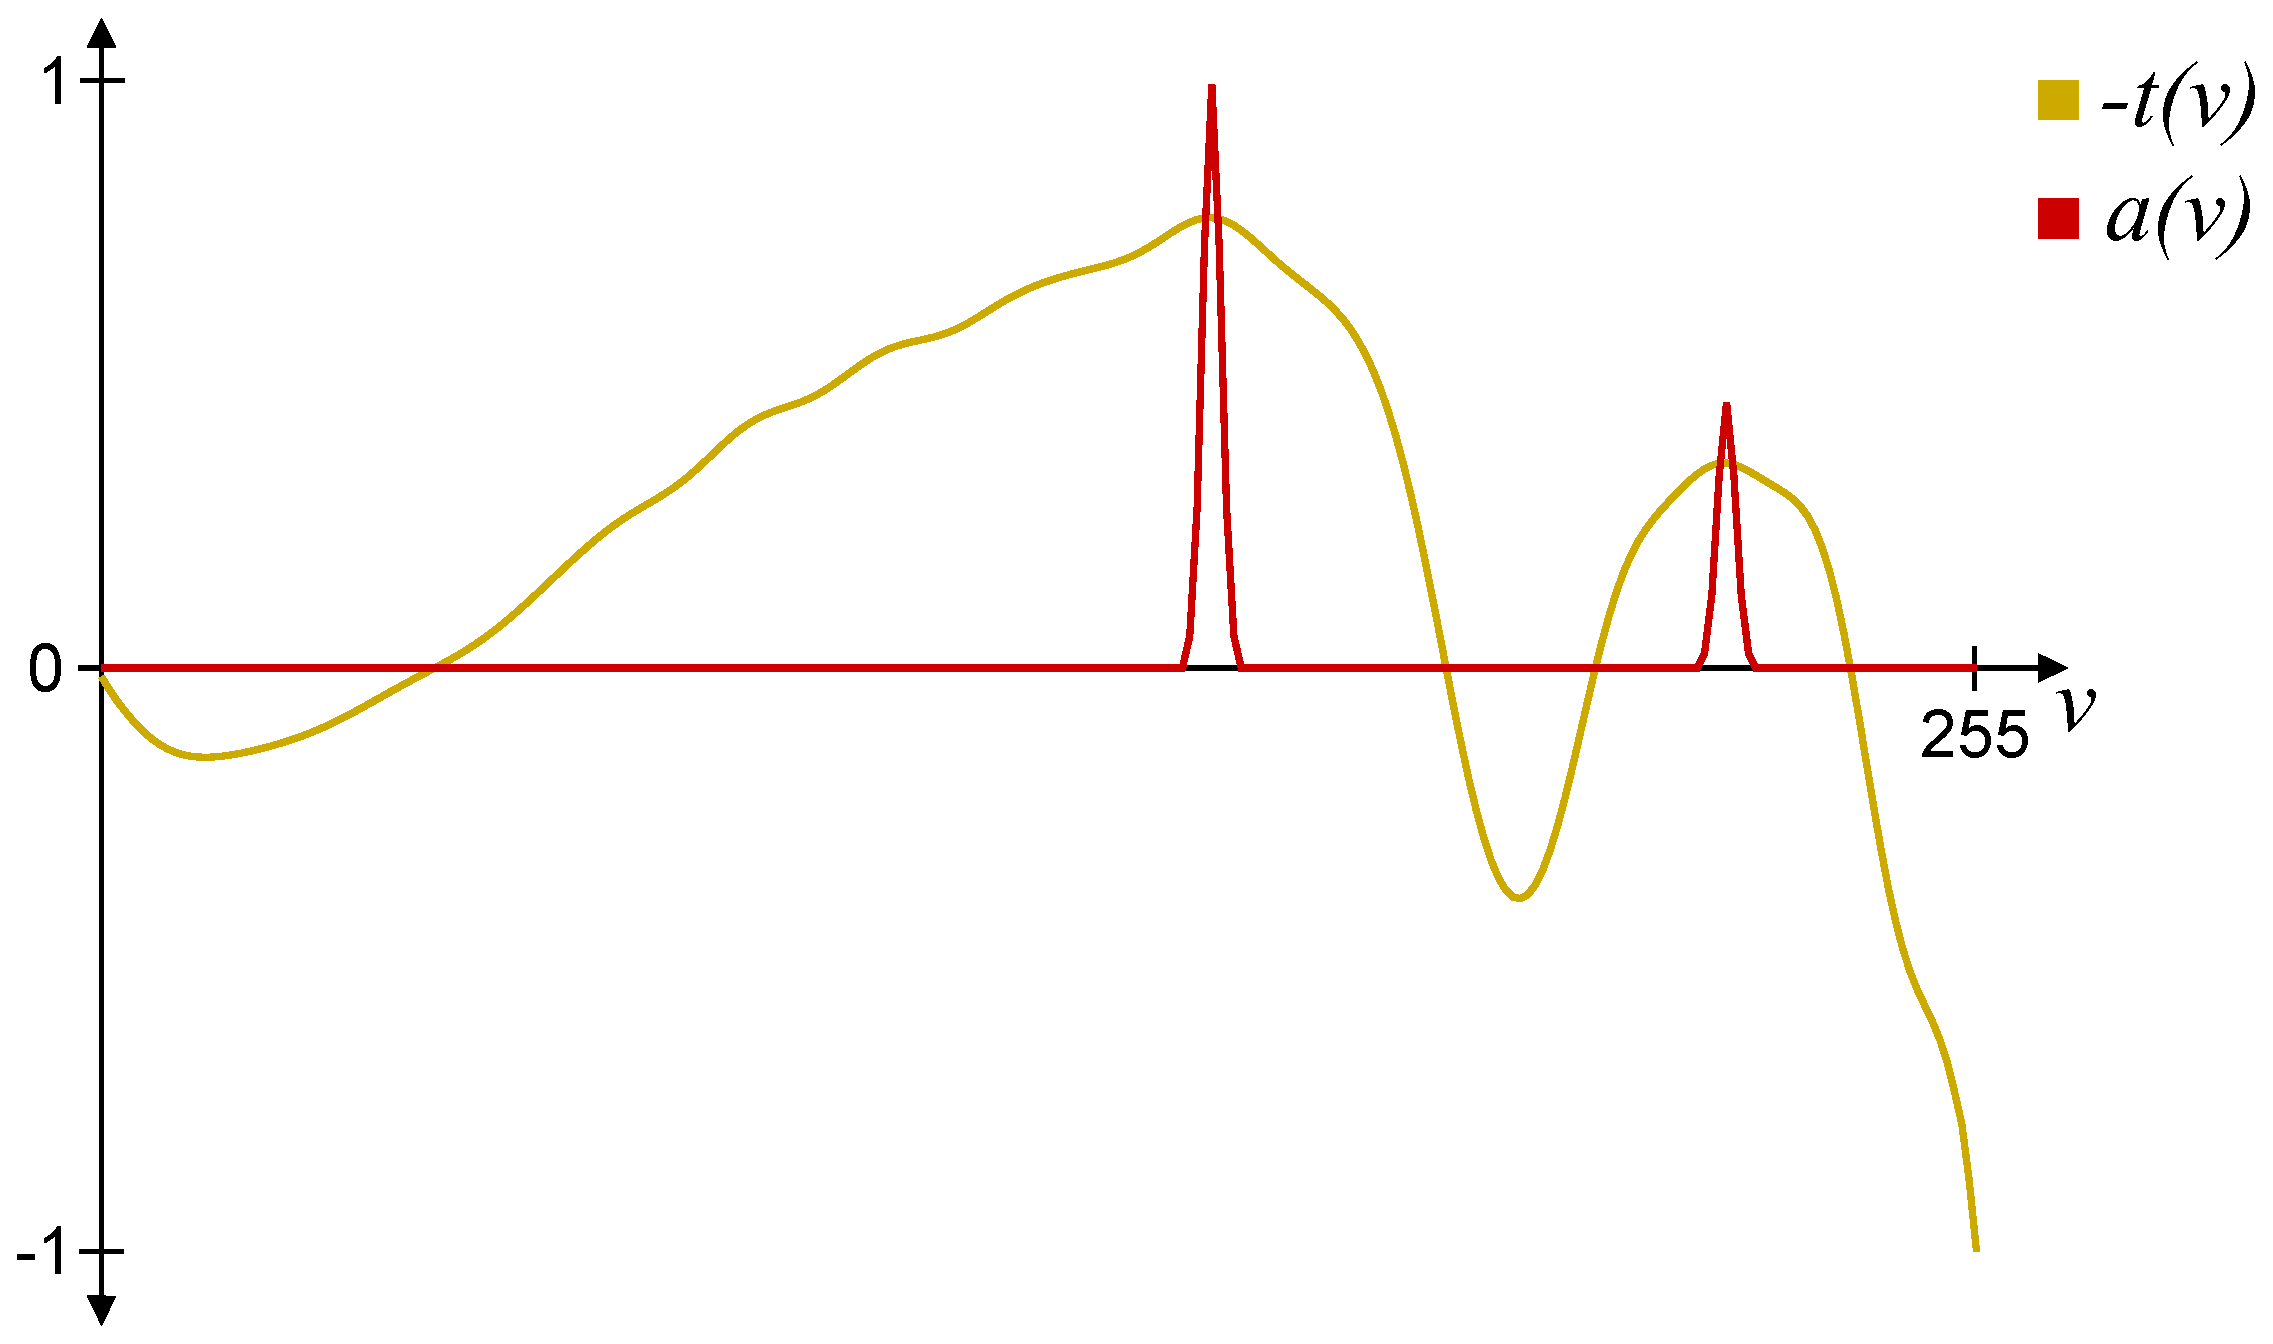
\includegraphics[width=0.65\textwidth]{images/r_m_nucleon_ft}			\label{fig:r_nucleon_mine}
	}
	\caption{Visualização e função de transferência do volume \quote{Nucleon}.}
	\label{fig:r_nucleon}
\end{figure}
	
%%%%%%%%%%%%%%%%%%%%%%%%%%%%%%%%%% ENGINE %%%%%%%%%%%%%%%%%%%%%%%%%%%%%%%%%%%%%
%	A Figura~\ref{fig:r_engine_slice} exibe uma fatia do volume \quote{Engine}, onde pode ser observada a existência de $ 3 $ fronteiras. Comparando as visualizações resultantes dos dois métodos, exibidas na Figura~\ref{fig:r_engine}, percebe-se que ambos foram capazes de realçar corretamente as fronteiras do volume. No entanto, ressalta-se que esta equivalência só foi possível após encontrar o valor de $ g_{thresh} $ que eliminou algumas regiões da visualização do método de \textit{Kindlmann e Durkin} que foram realçadas indevidamente, devido ao deslocamento do segundo pico da sua função de transferência.
%
%\begin{figure}[h]
%	\centering
%	\subfigure[Método de \textit{Kindlmann e Durkin}.]
%	{
%		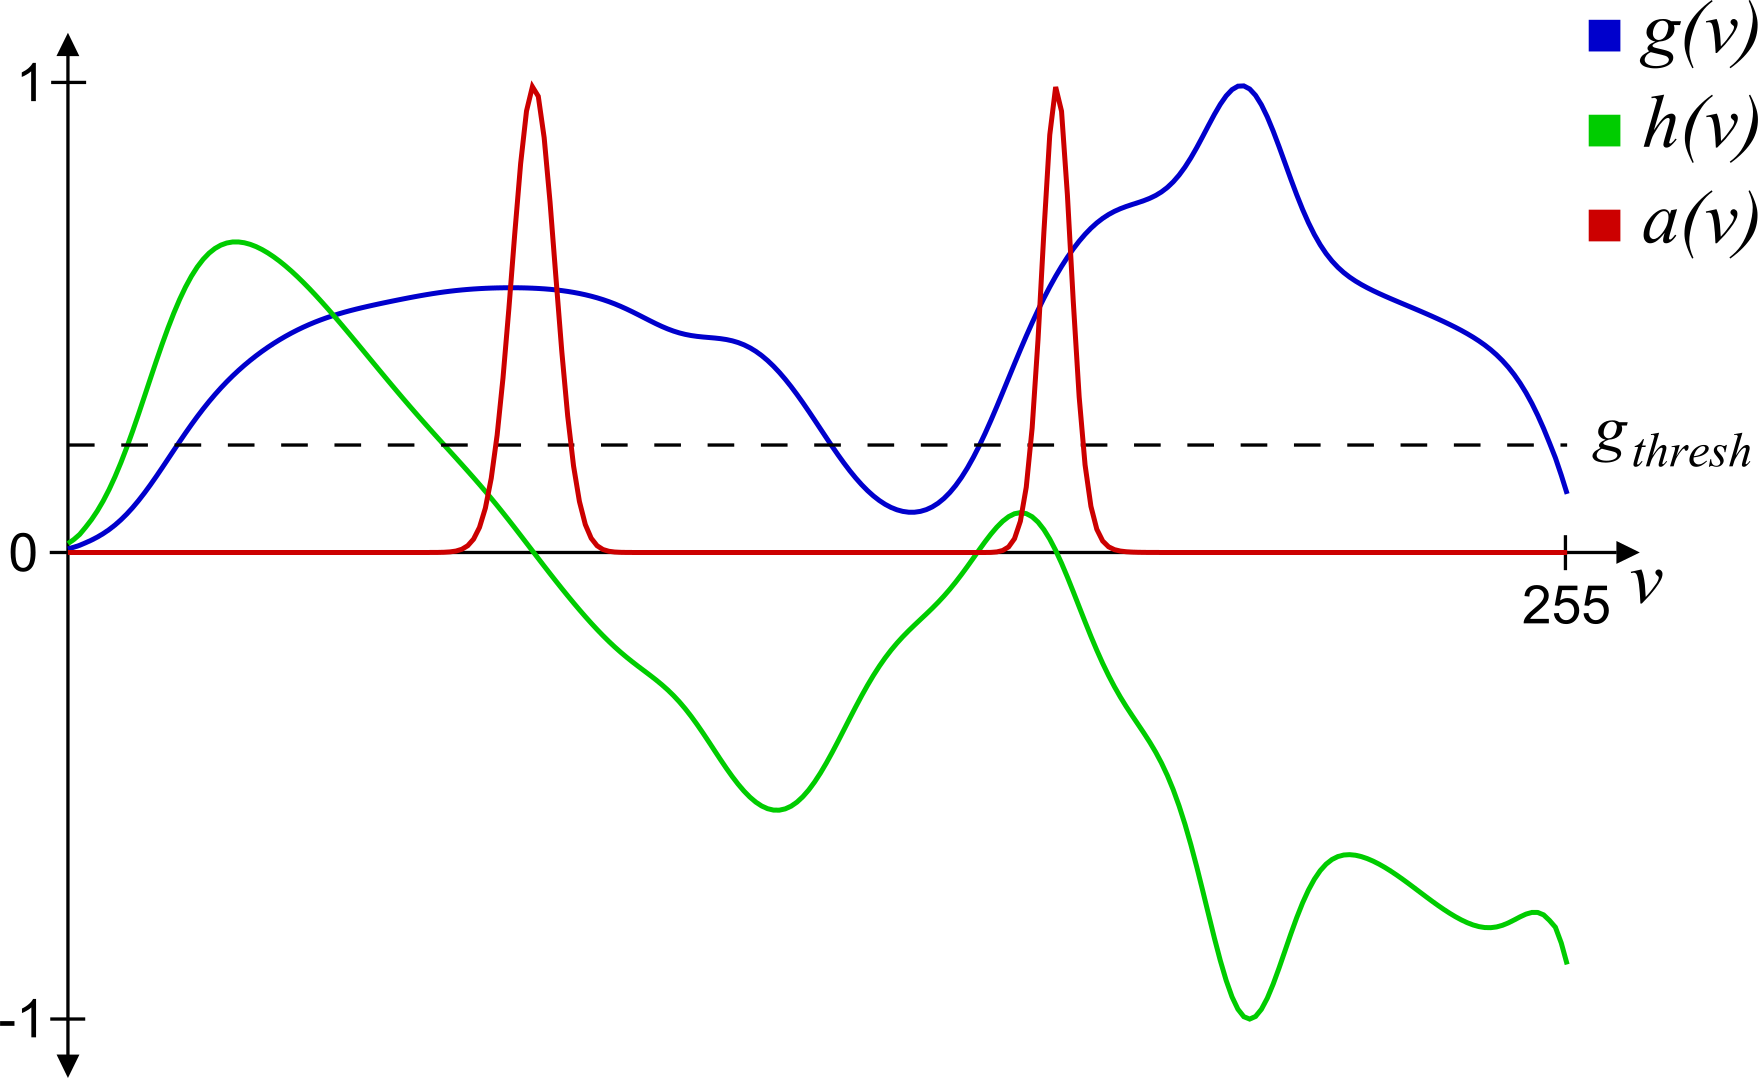
\includegraphics[width=0.35\textwidth]{images/r_g_engine}
%		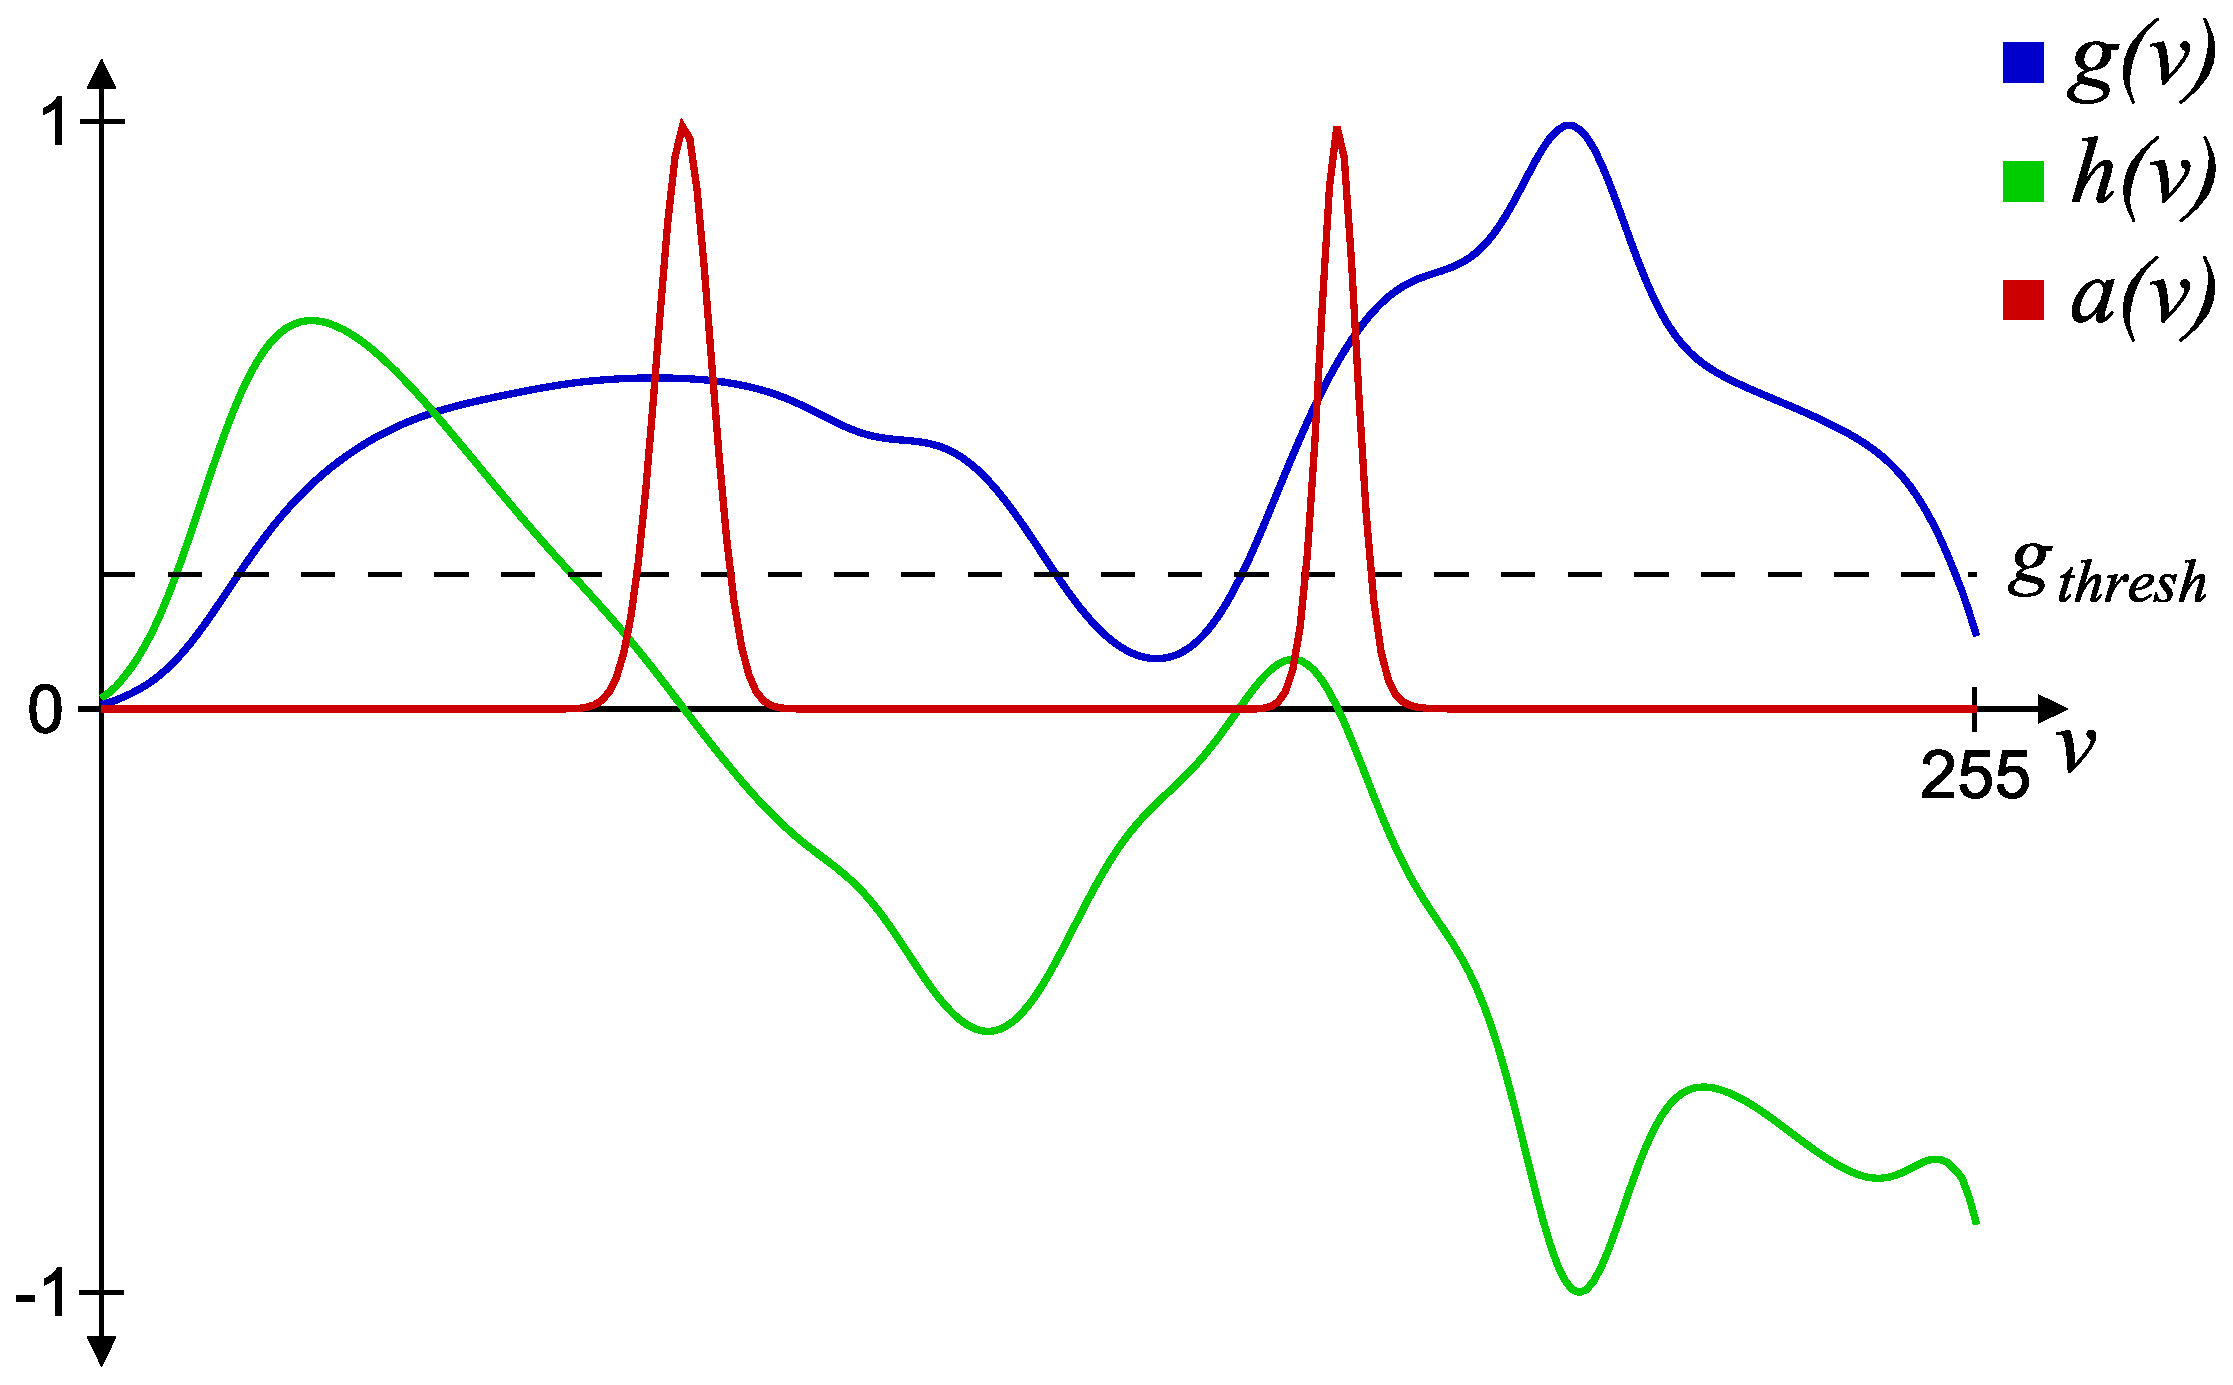
\includegraphics[width=0.65\textwidth]{images/r_g_engine_ft}
%		\label{fig:r_engine_kd}
%	}
%	\subfigure[Método proposto.]
%	{
%		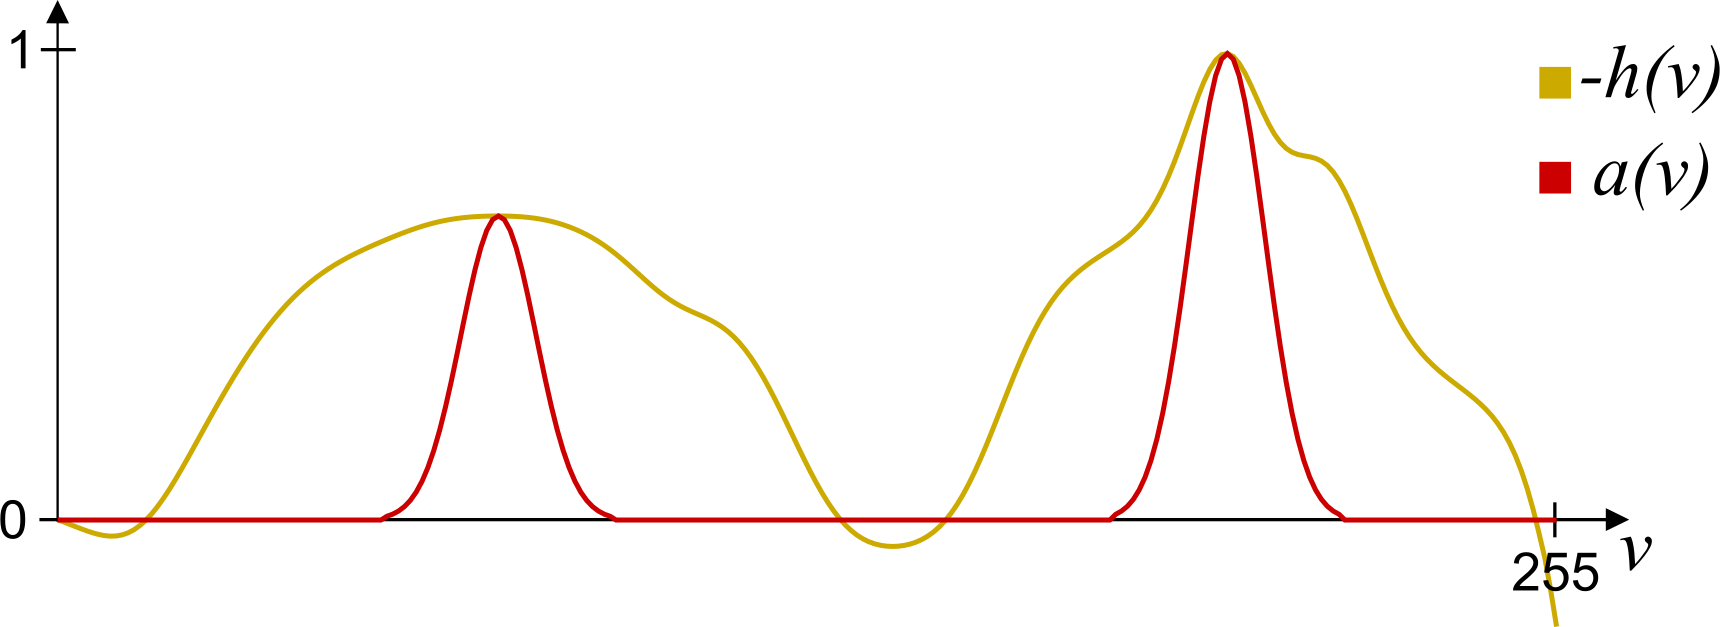
\includegraphics[width=0.35\textwidth]{images/r_m_engine}
%		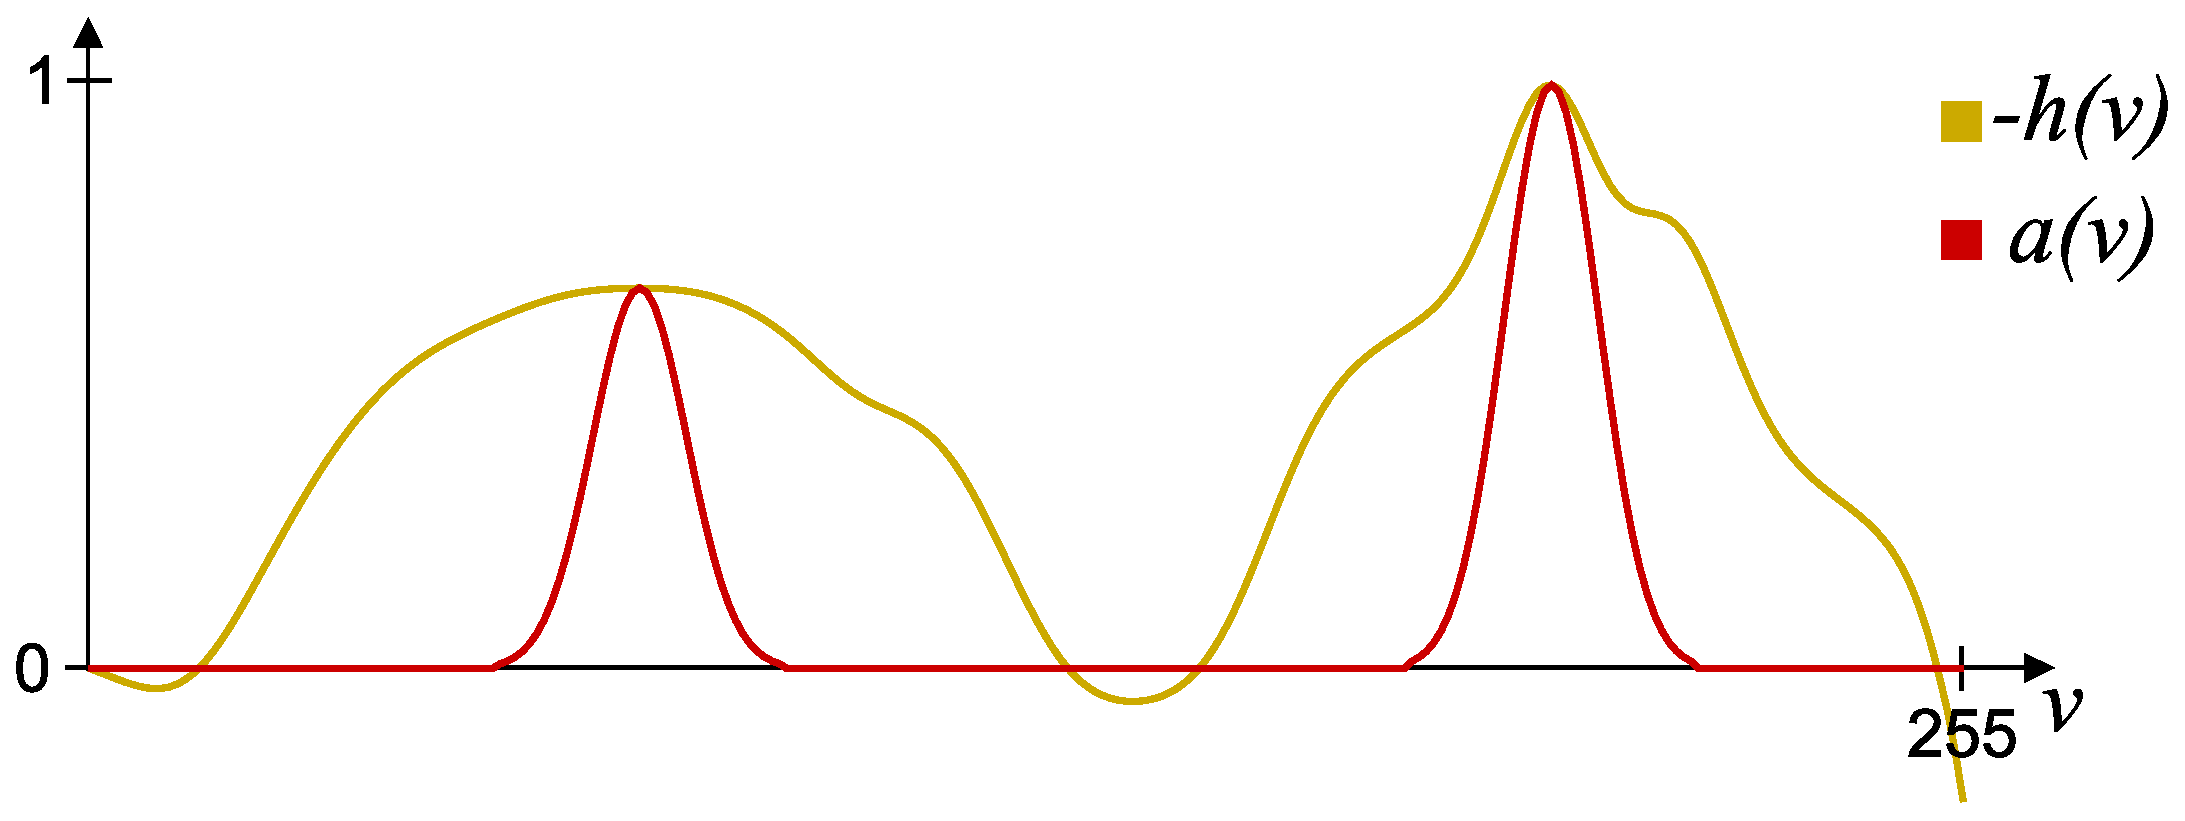
\includegraphics[width=0.65\textwidth]{images/r_m_engine_ft}			\label{fig:r_engine_mine}
%	}
%	\caption{Visualização e função de transferência do volume \quote{Engine}.}
%	\label{fig:r_engine}
%\end{figure}
%%%%%%%%%%%%%%%%%%%%%%%%%%%%%%%%%% CT HEAD %%%%%%%%%%%%%%%%%%%%%%%%%%%%%%%%%%%%%
	O volume a seguir é uma tomografia computadorizada de uma cabeça com uma estrutura de suporte na parte de trás. A Figura~\ref{fig:r_cthead} mostra que os dois métodos realçam a cabeça, o crânio e a estrutura de suporte. O segundo pico das duas funções de transferência são coincidentes e equivalem ao crânio, em amarelo. No entanto, o primeiro pico não coincide.
	
	O método de \textit{Kindlmann~e~Durkin} apresenta um deslocamento para a esquerda, centralizando esse pico onde a segunda derivada é igual a zero. Devido à posição desse pico (que não ocorre junto a um máximo local na primeira derivada média), alguns voxels do volume são realçados juntamente com a cabeça e sua estrutura de suporte, permitindo a interpretação de que todos compõem uma só isosuperfície. O mesmo não ocorre com o método proposto por esta dissertação, que realça a cabeça corretamente ao mesmo tempo que mostra menos a estrutura presente na sua parte de trás, permitindo entendê-las como isosuperfícies diferentes.

\begin{figure}[h]
	\centering
	\subfigure[Método de \textit{Kindlmann e Durkin}.]
	{
		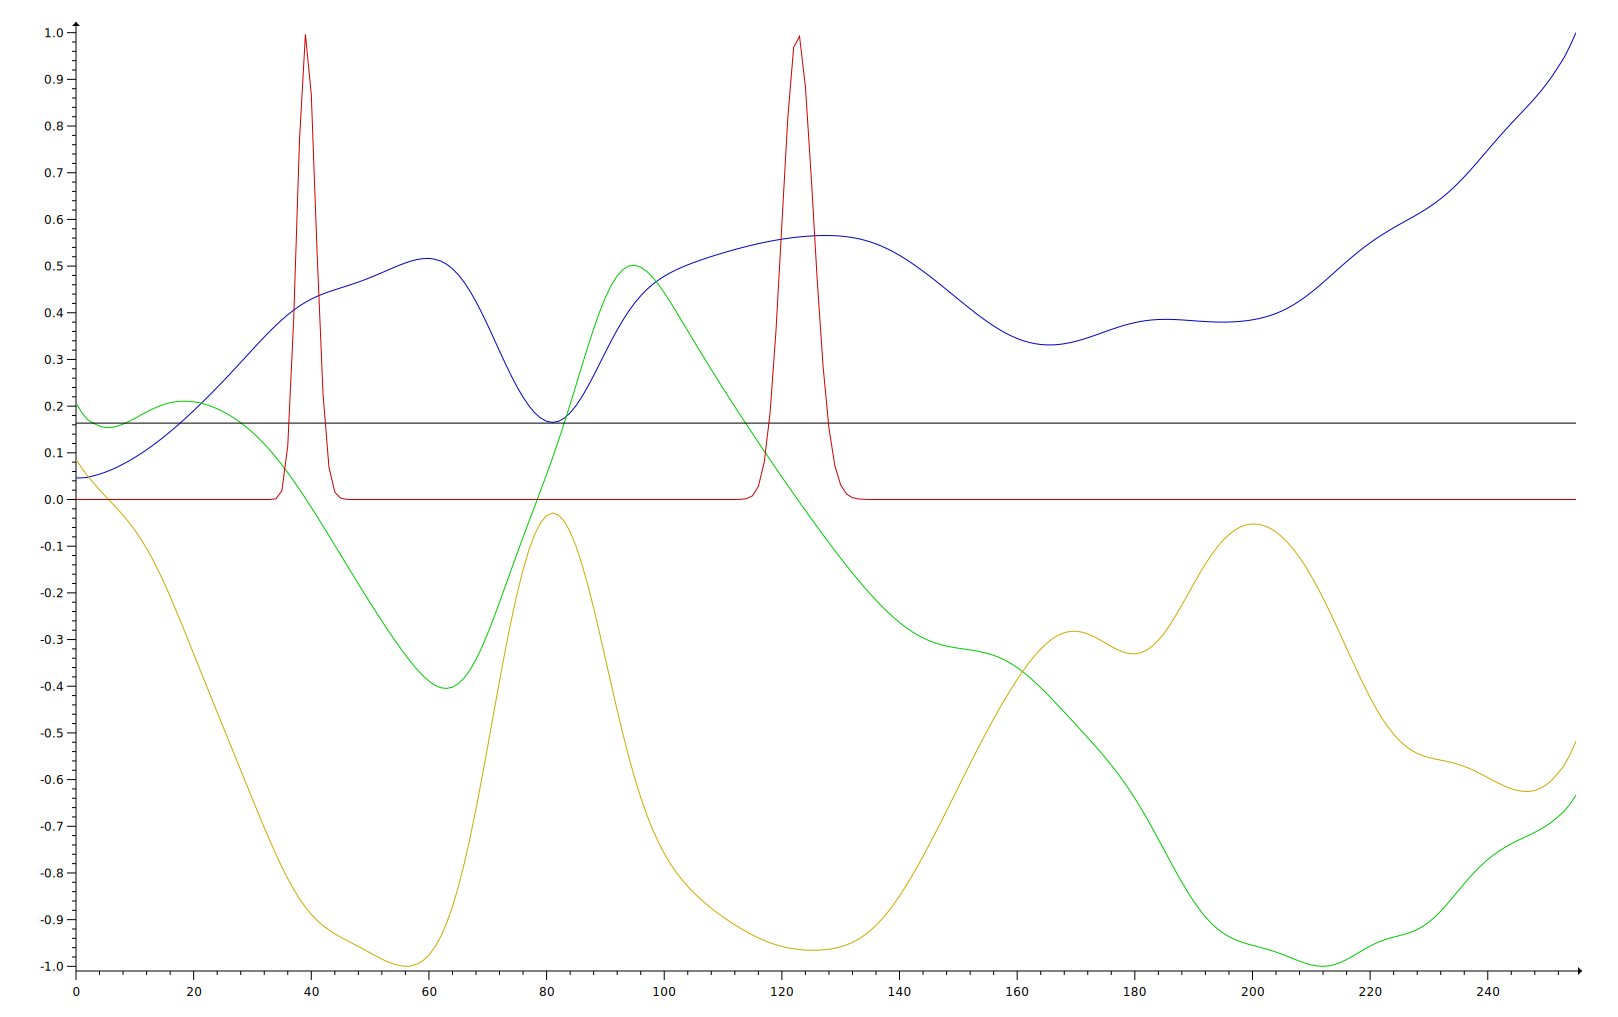
\includegraphics[width=0.35\textwidth]{images/r_g_cthead}
		\includegraphics[width=0.65\textwidth]{images/r_g_cthead_ft}
		\label{fig:r_cthead_kd}
	}
	\subfigure[Método proposto.]
	{
		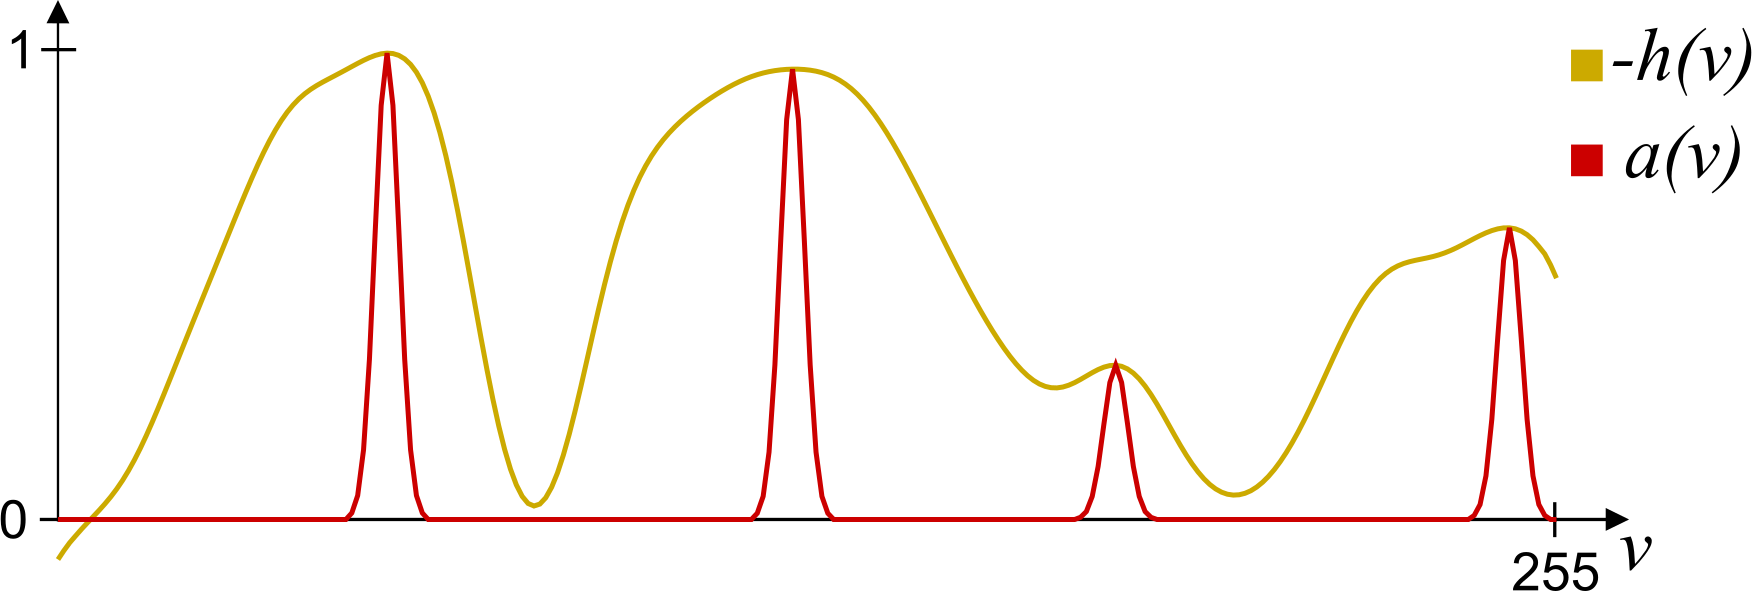
\includegraphics[width=0.35\textwidth]{images/r_m_cthead}
		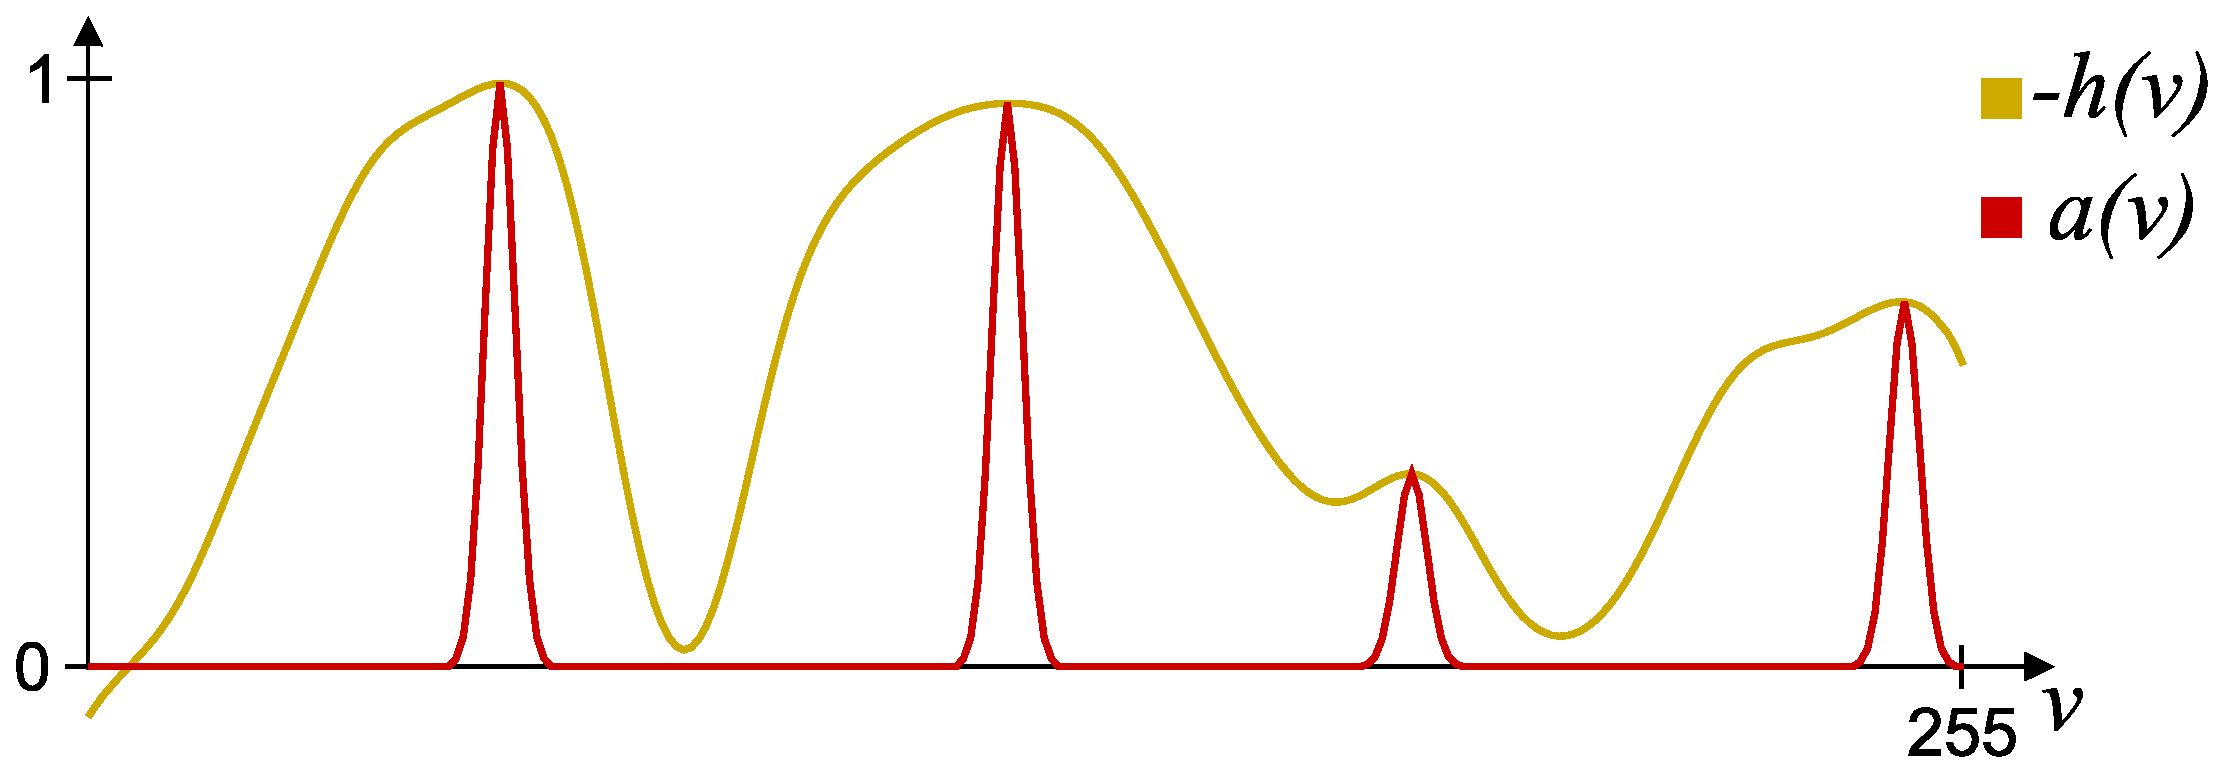
\includegraphics[width=0.65\textwidth]{images/r_m_cthead_ft}			\label{fig:r_cthead_mine}
	}
	\caption{Visualização e função de transferência do volume \quote{CT Head}.}
	\label{fig:r_cthead}
\end{figure}

	O terceiro pico da função de transferência na Figura~\ref{fig:r_cthead}~\ref{fig:r_cthead_mine} destaca incorretamente uma isosuperfície, pois ela não corresponde a uma fronteira. Ao isolá-la, vê-se uma estrutura semelhante ao crânio, porém incompleta. Já a quarta fronteira foi obtida corretamente e realça os dentes. A Figura~\ref{fig:r_cthead_iso} mostra a visualização apenas do crânio, que pode ser obtida através da interface, selecionando apenas a segunda fronteira.

\begin{figure}[h]
	\centering
	\subfigure[Função de transferência.]
	{
		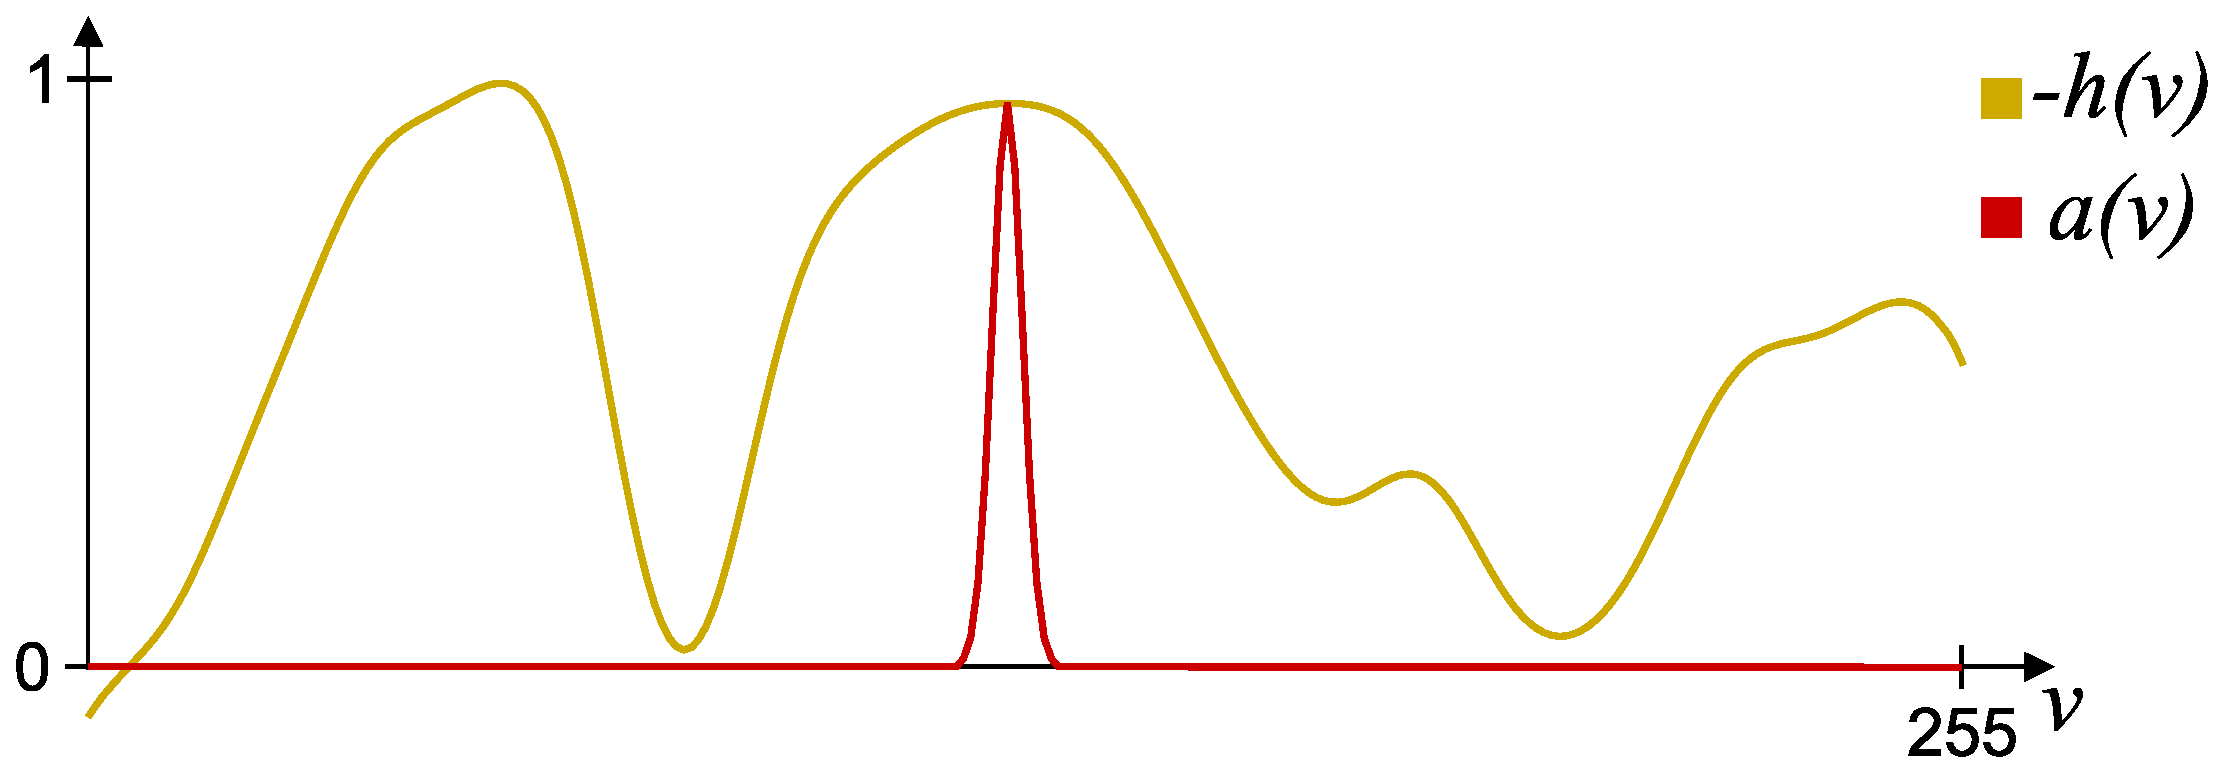
\includegraphics[width=0.8\textwidth]{images/r_m_cthead_iso_ft}
	}
	\subfigure[Visualização volumétrica.]
	{
		\includegraphics[width=0.7\textwidth]{images/r_m_cthead_iso}
	}
	\caption{Realce do crânio do volume \quote{CT Head} através da interface.}
	\label{fig:r_cthead_iso}
\end{figure}

%%%%%%%%%%%%%%%%%%%%%%%%%%%%%%%%%% Tooth %%%%%%%%%%%%%%%%%%%%%%%%%%%%%%%%%%%%%

	O volume seguinte é um dente envolvido por um material que causa a forma cilíndrica revelada nas visualizações da Figura~\ref{fig:r_tooth}. Como pode ser observado, tanto as funções de transferência como suas respectivas visualizações são semelhantes em ambos os métodos. Percebe-se apenas um ligeiro deslocamento da última fronteira obtida pelo método de \textit{Kindlmann~e~Durkin}, resultando em uma isosuperfície laranja mais forte que a encontrada pelo método aqui proposto.
	
\begin{figure}[h]
	\centering
	\subfigure[Método de \textit{Kindlmann e Durkin}.]
	{
		\includegraphics[width=0.35\textwidth]{images/r_g_tooth}
		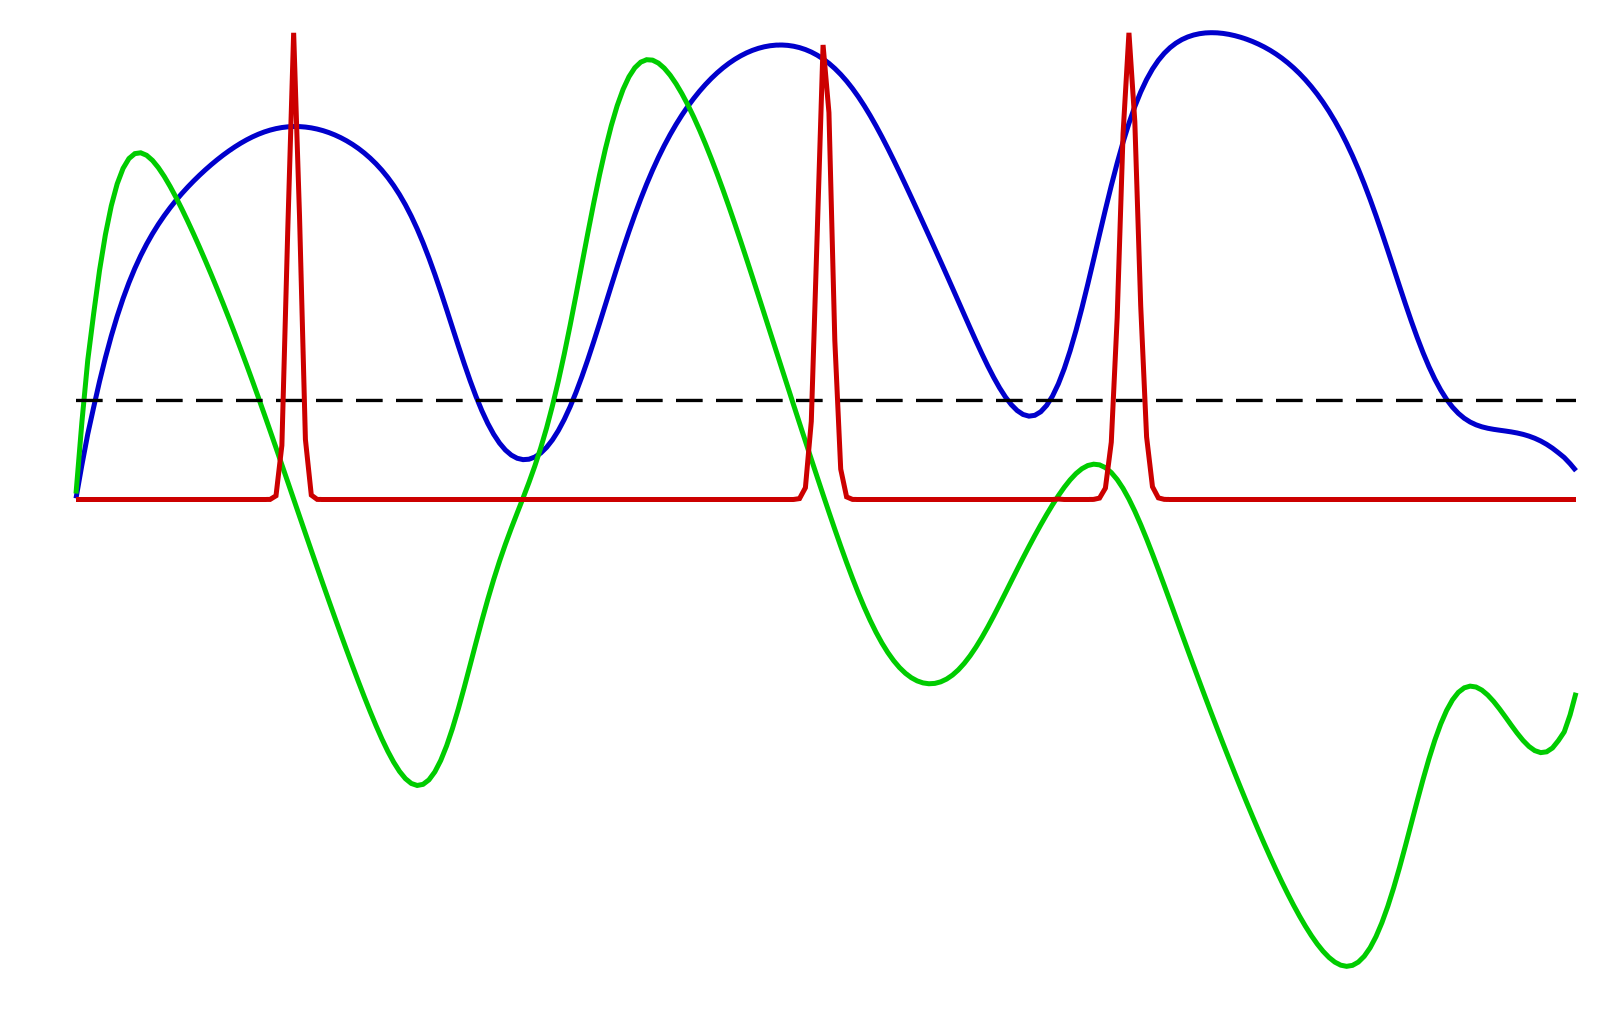
\includegraphics[width=0.65\textwidth]{images/r_g_tooth_ft}
		\label{fig:r_tooth_kd}
	}
	\subfigure[Método proposto.]
	{
		\includegraphics[width=0.35\textwidth]{images/r_m_tooth}
		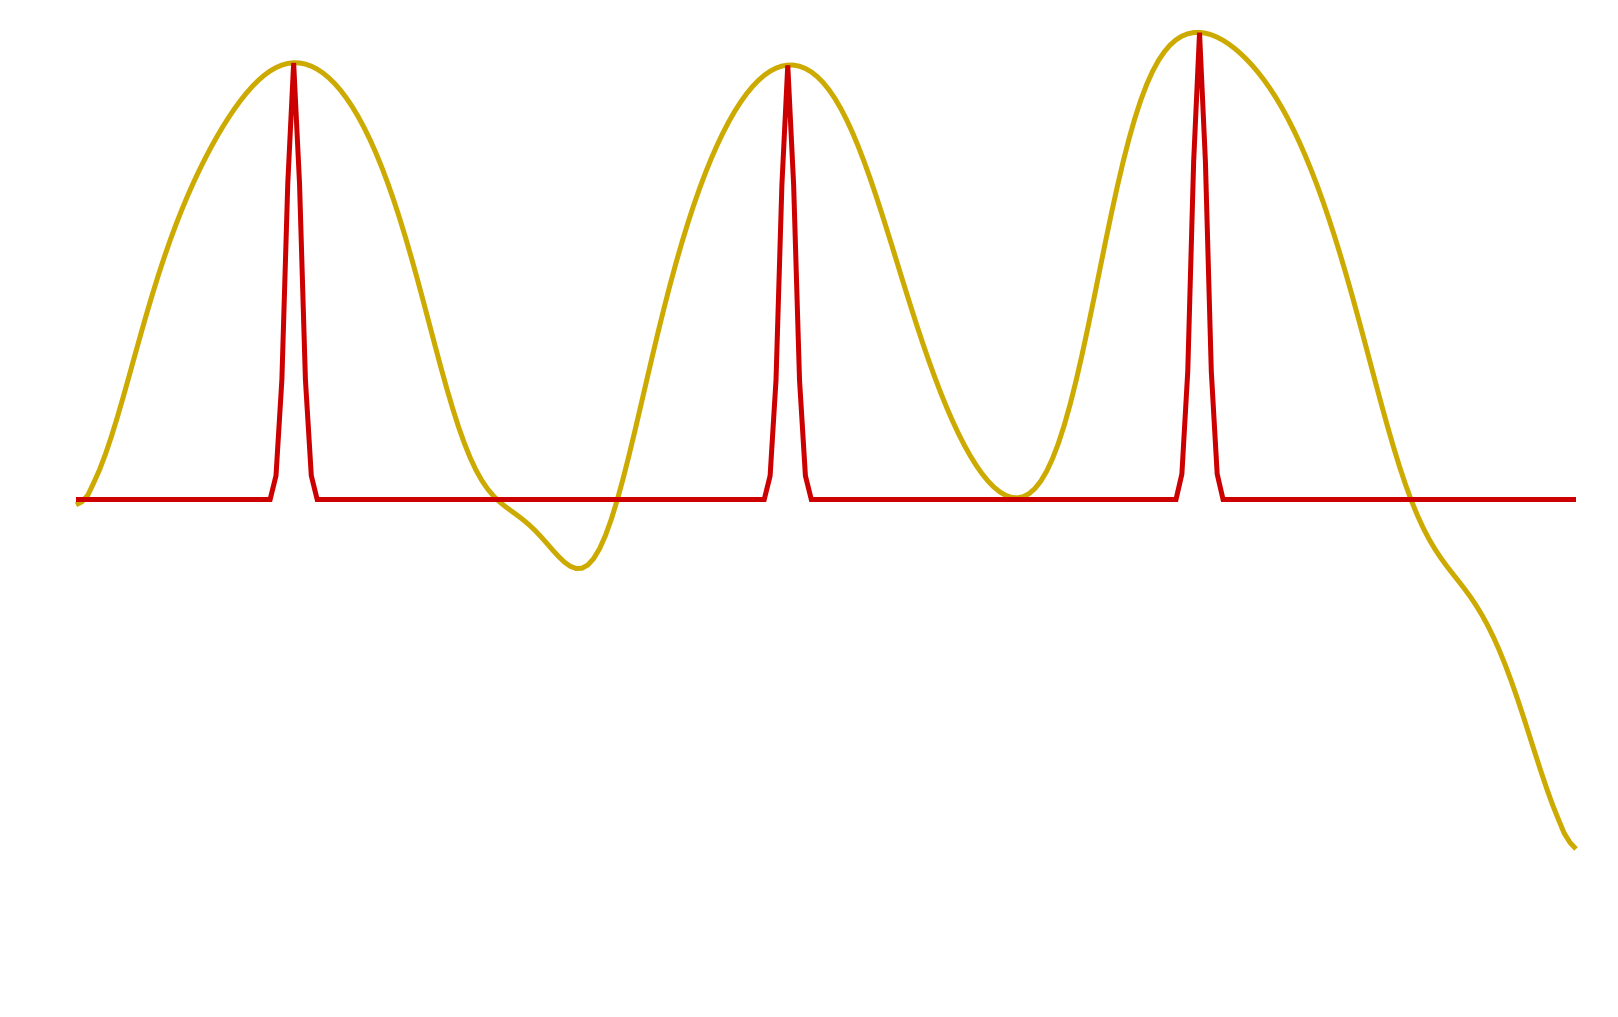
\includegraphics[width=0.65\textwidth]{images/r_m_tooth_ft}			\label{fig:r_tooth_mine}
	}
	\caption{Visualização e função de transferência de um dente.}
	\label{fig:r_tooth}
\end{figure}

%%%%%%%%%%%%%%%%%%%%%%%%%%%%%%%%%% Bonsai %%%%%%%%%%%%%%%%%%%%%%%%%%%%%%%%%%%%%
	O bonsai já é um volume conhecido na literatura, principalmente pelo ruído presente acima das raízes, que possui valor muito próximo ao das folhas. Portanto, para visualizá-lo corretamente, é preciso remover as isosuperfícies que correspondem a esse ruído e aumentar a largura da função de transferência até que até que as folhas apareçam novamente. No método 1D de \textit{Kindlmann~e~Durkin} esse processo é feito através do $ g_{thresh} $, enquanto no método desta dissertação desliga-se as isosuperfícies através da interface, como já explicado na Seção~\ref{sec:my.tf}.
	
	Como pode ser observado na Figura~\ref{fig:r_m_bonsai}, as funções de transferência são bem distintas, apesar de resultarem em visualizações quase idênticas. Então, cabe observar que, dentro da proposta de realçar como fronteira a isosuperfície que possui maior derivada, o método proposto por esta dissertação apresenta uma função de transferência mais adequada.
	
\begin{figure}[h]
	\centering
	\subfigure[Método de \textit{Kindlmann e Durkin}.]
	{
		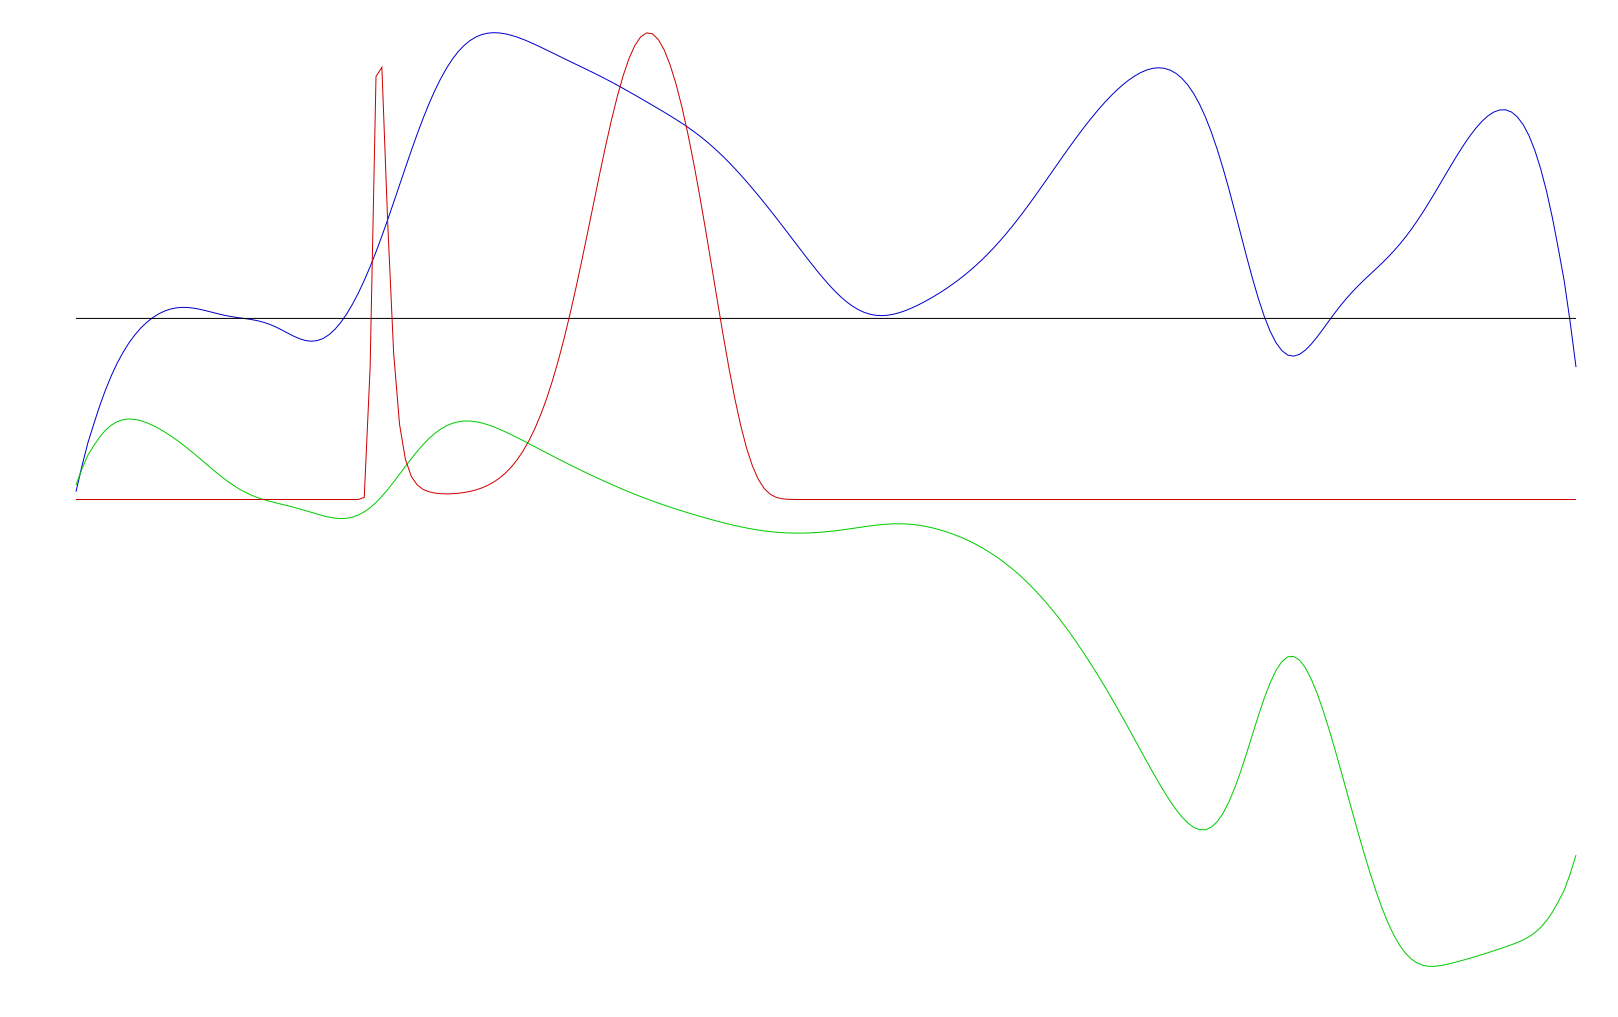
\includegraphics[width=0.7\textwidth]{images/r_g_bonsai_ft}
		\label{fig:r_bonsai_kd_ft}
	}
	\subfigure[Método proposto.]
	{
		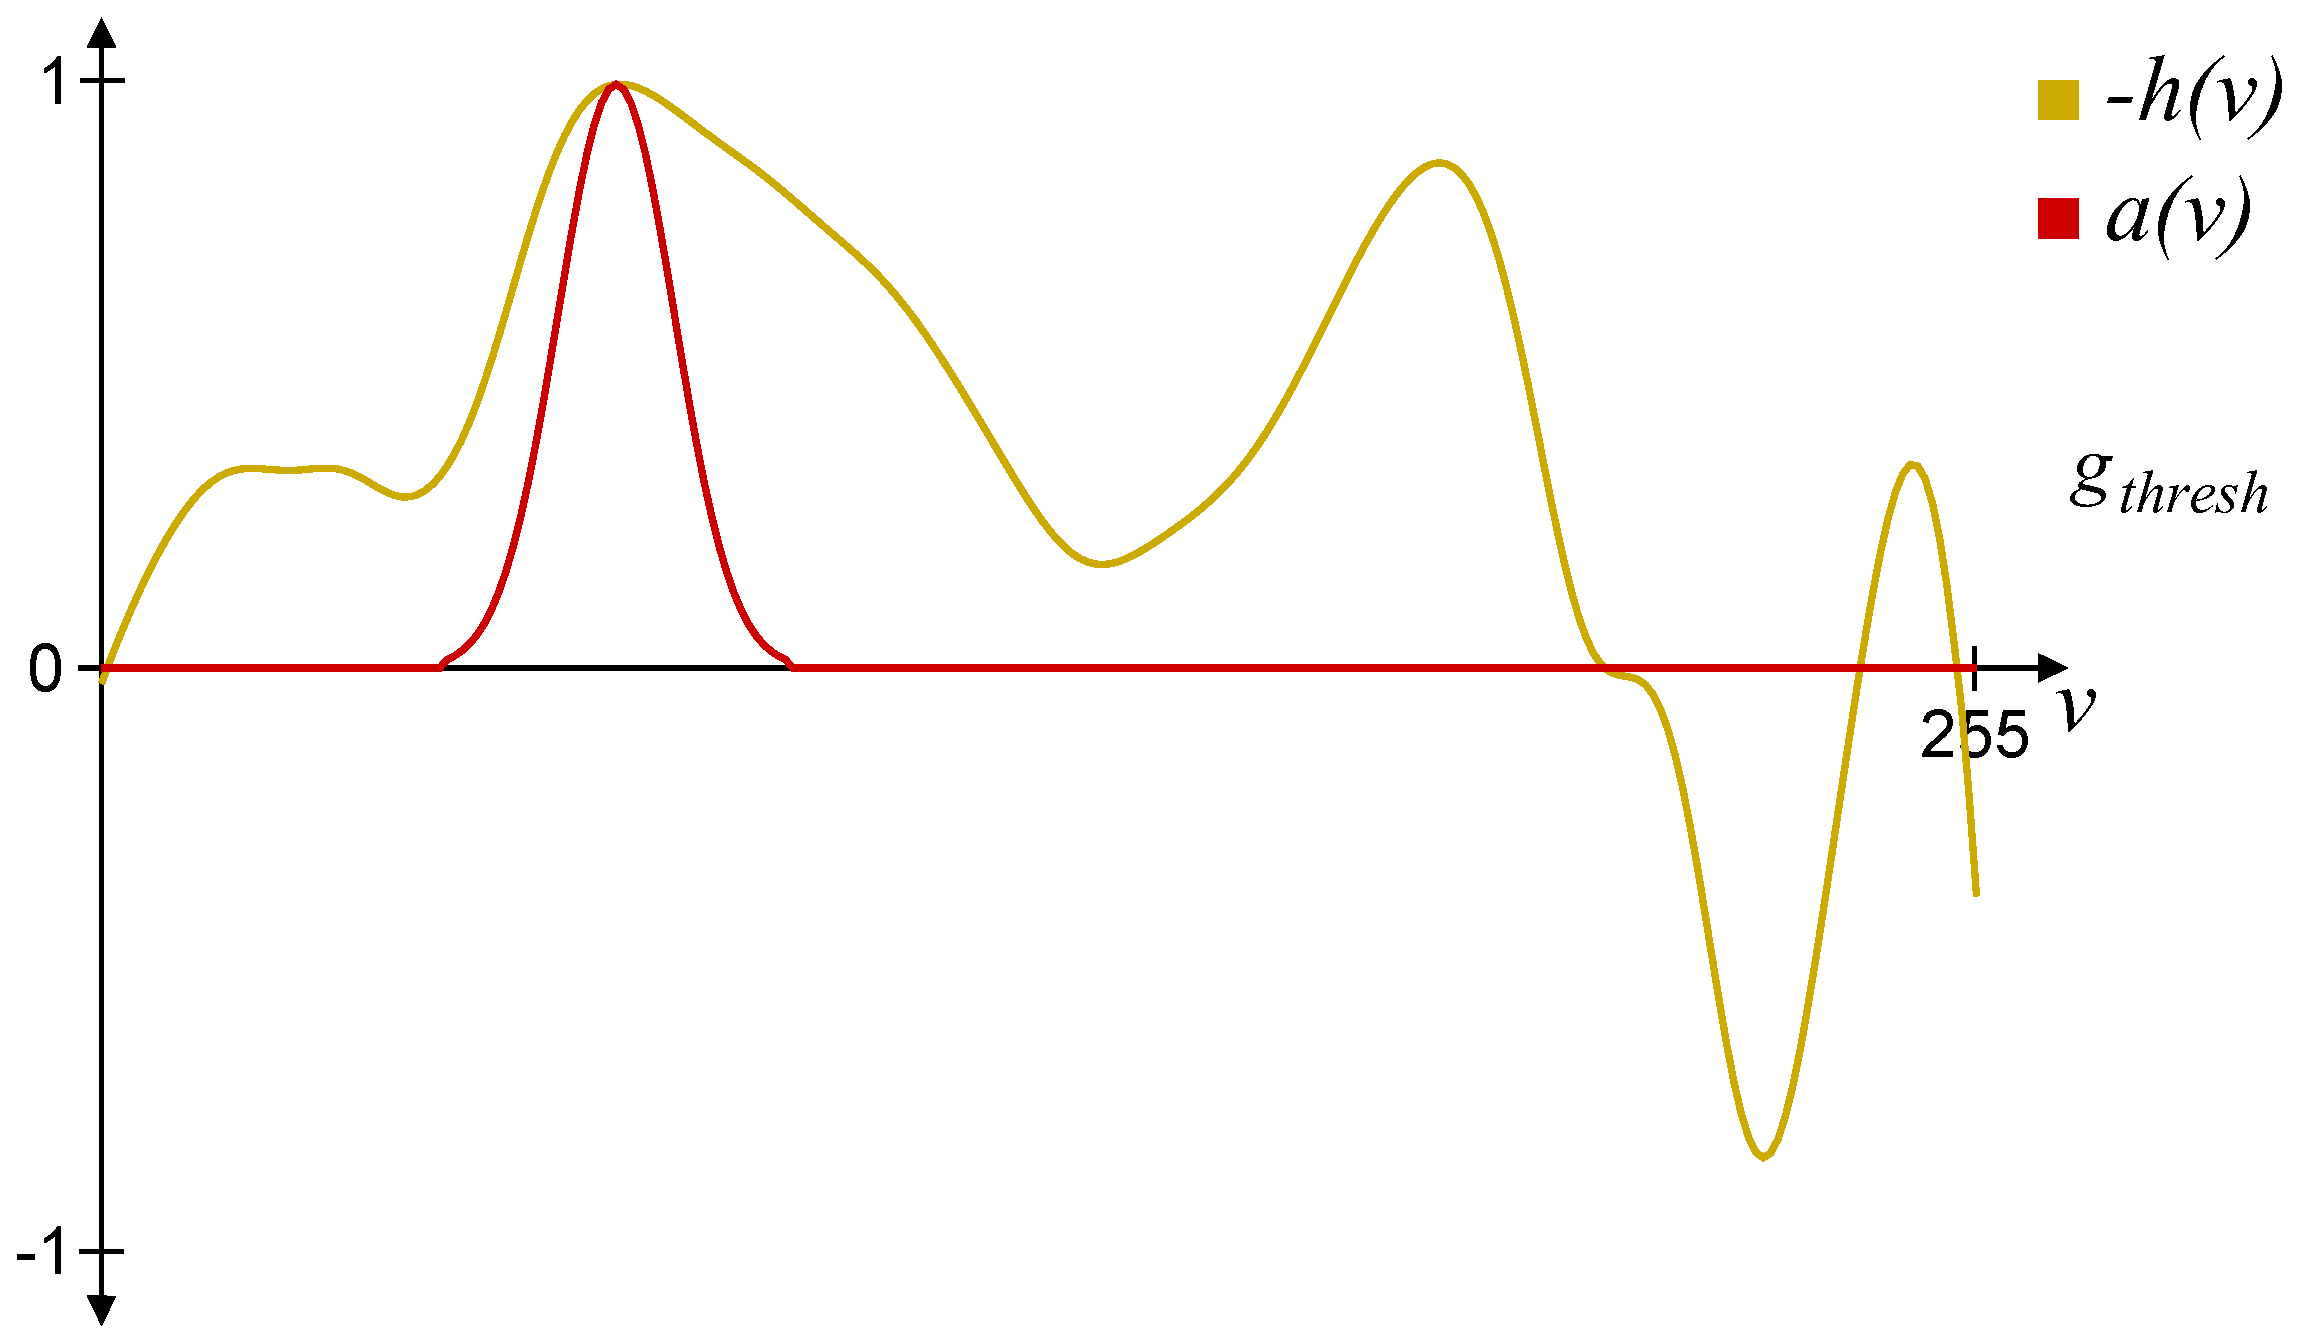
\includegraphics[width=0.7\textwidth]{images/r_m_bonsai_ft}			\label{fig:r_bonsai_mine_ft}
	}
	\subfigure[Método de \textit{Kindlmann e Durkin}.]
	{
		\includegraphics[width=0.47\textwidth]{images/r_g_bonsai}
		\label{fig:r_bonsai_kd}
	}
	\subfigure[Método proposto.]
	{
		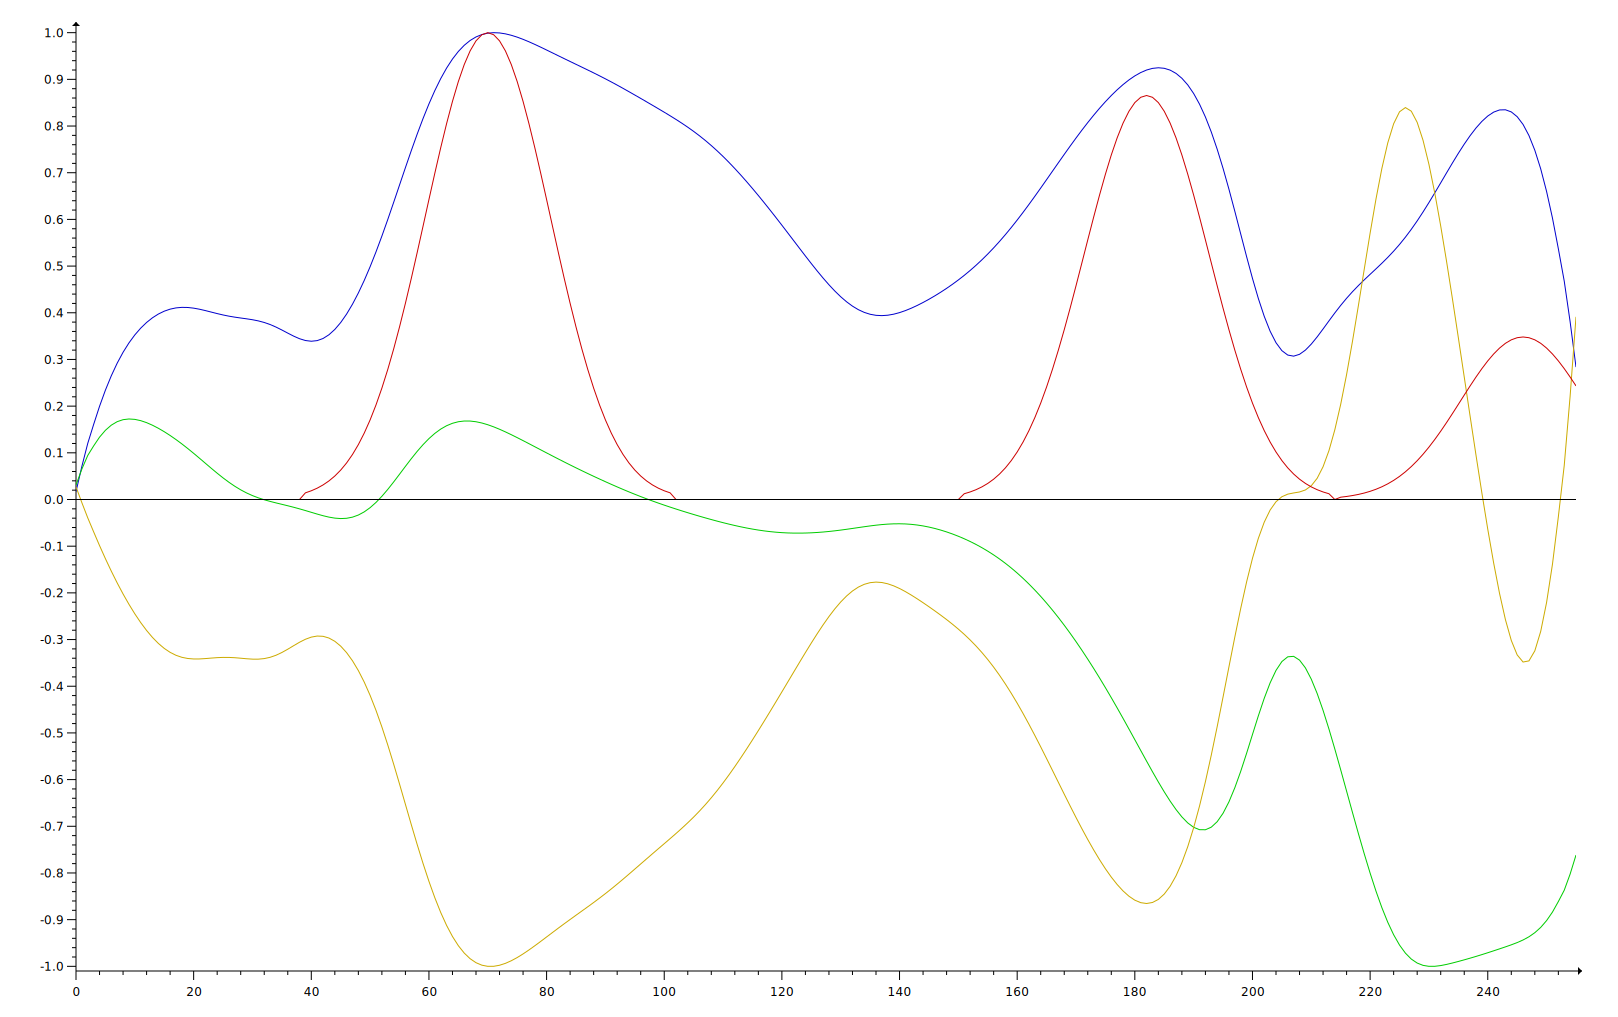
\includegraphics[width=0.47\textwidth]{images/r_m_bonsai}
		\label{fig:r_bonsai_mine}
	}
	\caption{Visualização e função de transferência do bonsai.}
	\label{fig:r_m_bonsai}
\end{figure}

%%%%%%%%%%%%%%%%%%%%%%%%%%%%%%%%%% X %%%%%%%%%%%%%%%%%%%%%%%%%%%%%%%%%%%%%
\clearpage
	Os dois volumes seguintes apresentam a mesma situação ocorrida com o bonsai no momento de comparar os dois métodos: funções de transferência diferentes que resultam em visualizações muito parecidas. Por isso, serão apresentados apenas os resultados oriundos do método proposto nesta dissertação.
	
	A Figura~\ref{fig:r_m_carp} mostra a função de transferência obtida com o método desta dissertação, bem como a visualização volumétrica resultante. As duas primeiras fronteiras vistas na FT correspondem respectivamente ao exterior e ao exoesqueleto da carpa. As outras duas representam regiões pequenas do exoesqueleto de maior intensidade. A Figura~\ref{fig:r_m_carp}~\ref{fig:r_m_carp_exo} mostra apenas o exoesqueleto da carpa. Para isso, a fronteira referente ao exterior da carpa foi desligada e a opacidade máxima da função de transferência aumentada.
	
\begin{figure}[h]
	\centering
	\subfigure[]
	{
		\includegraphics[width=0.7\textwidth]{images/r_m_carp_ft}
		\label{fig:r_m_carp_ft}
	}
	\subfigure[]
	{
		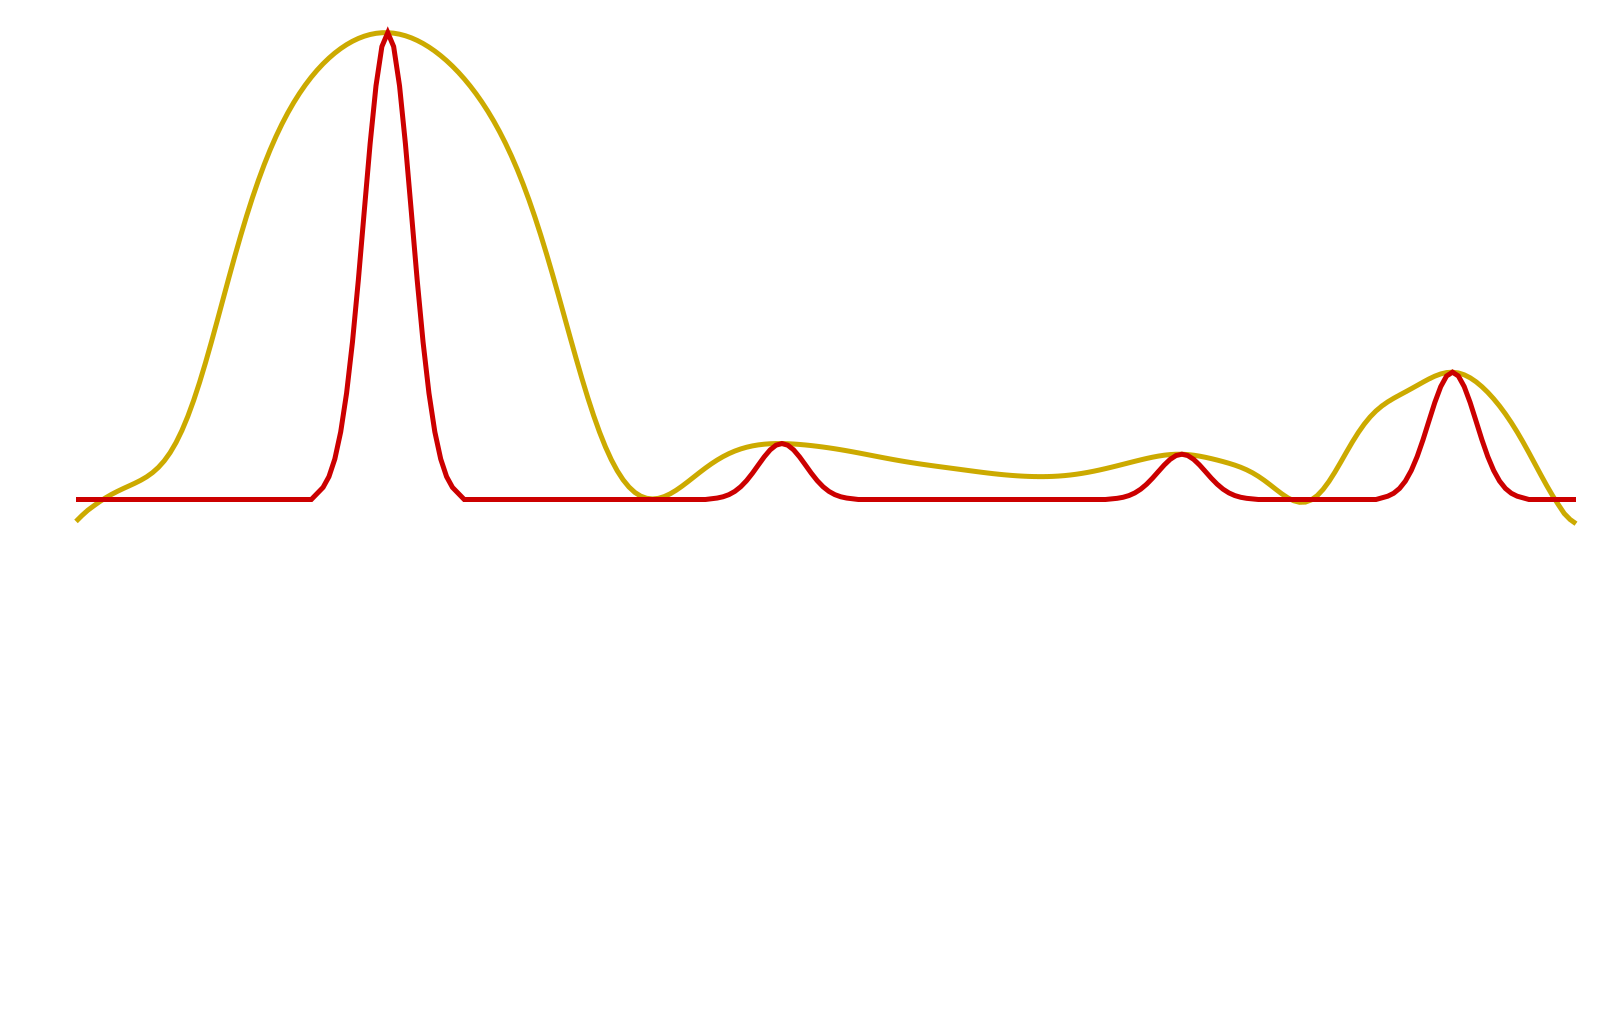
\includegraphics[width=0.8\textwidth]{images/r_m_carp}
		\label{fig:r_m_carp_side}
	}
	\subfigure[]
	{
		\includegraphics[width=0.8\textwidth]{images/r_m_carp_up}
		\label{fig:r_m_carp_up}
	}
	\subfigure[]
	{
		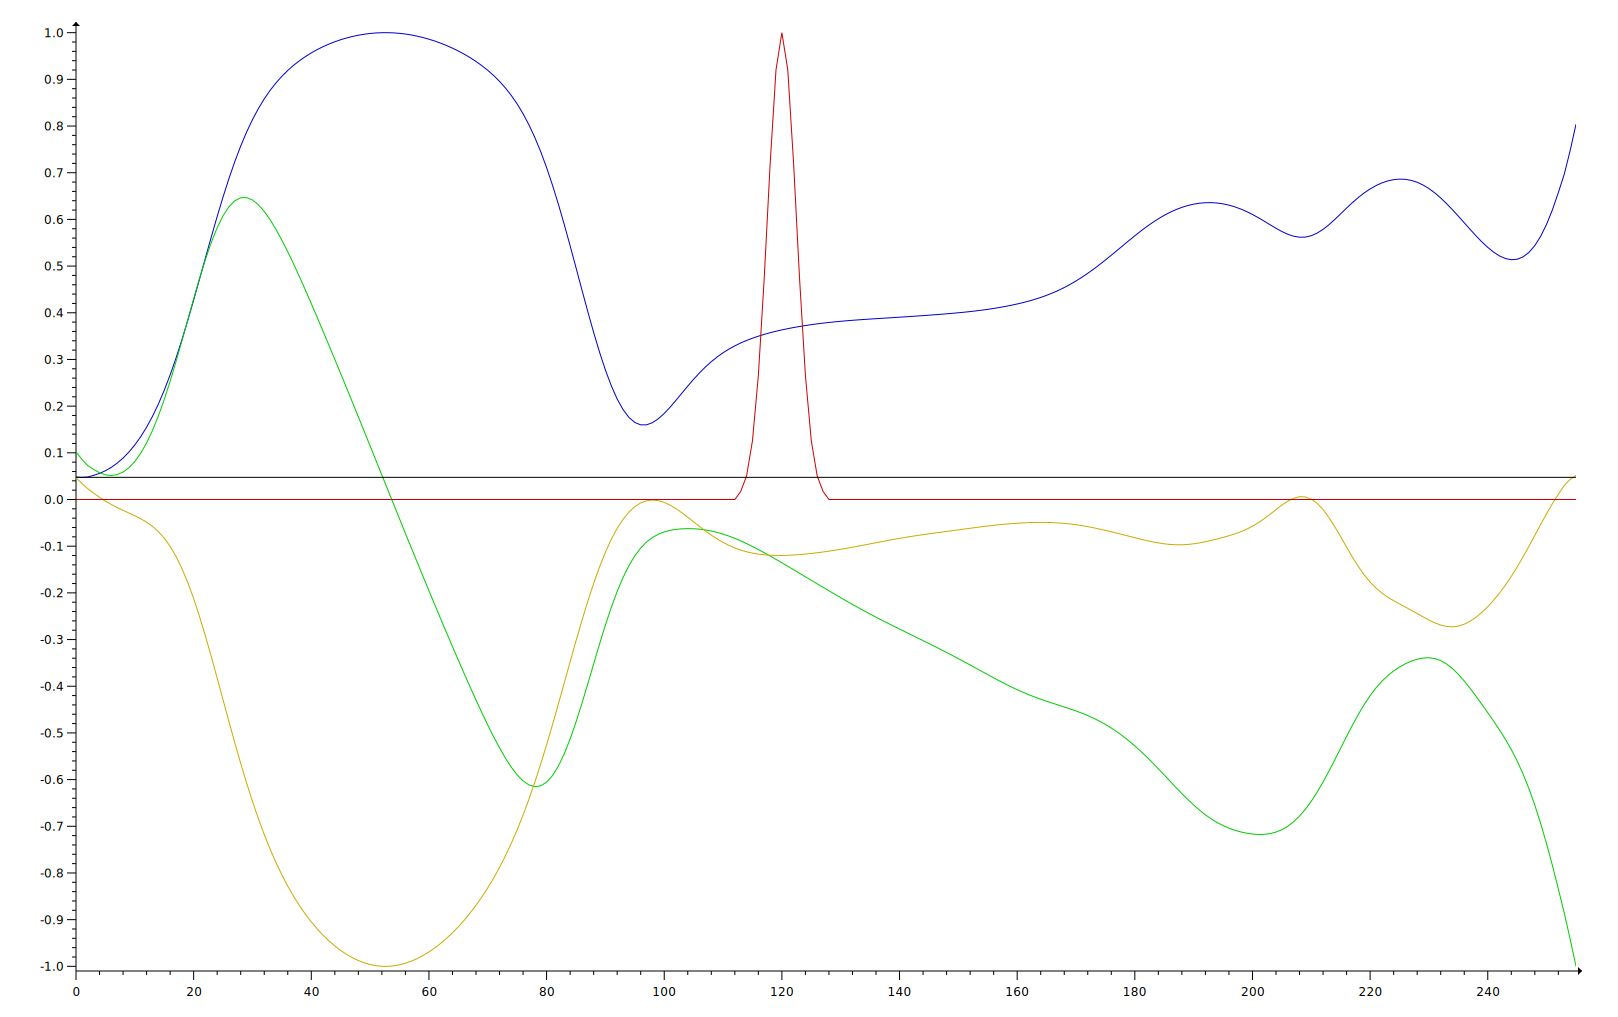
\includegraphics[width=0.8\textwidth]{images/r_m_carp_exo}
		\label{fig:r_m_carp_exo}
	}
	\caption{Carpa.}
	\label{fig:r_m_carp}
\end{figure}

%\begin{figure}[h]
%	\centering
%	\subfigure[]
%	{
%		\includegraphics[width=0.7\textwidth]{images/r_m_carp_exo_ft}
%	}
%	\subfigure[]
%	{
%		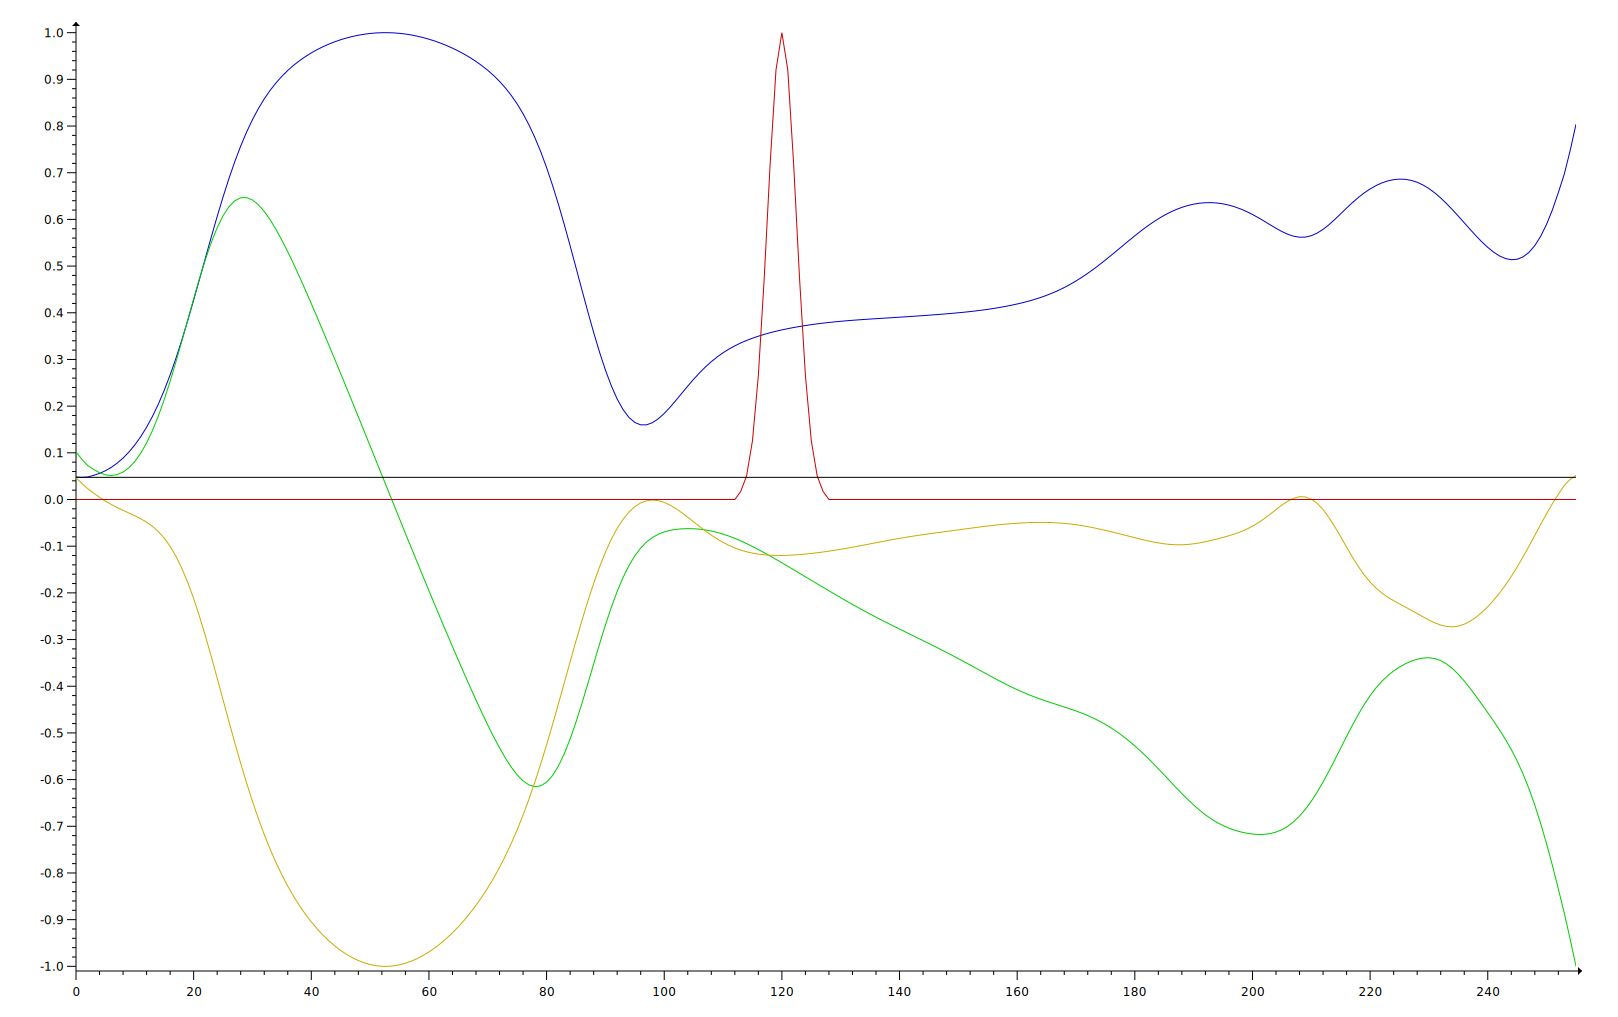
\includegraphics[width=0.8\textwidth]{images/r_m_carp_exo}
%	}	
%	\caption{Exoesqueleto da carpa.}
%	\label{fig:r_m_carp_exo}
%\end{figure}

	No volume \quote{Knee}, assim como no bonsai, foi preciso manipular a função de transferência em ambos os métodos para se obter apenas o osso. Então, desligou-se o pico da função de transferência que não correspondia aos ossos dos joelhos. Como neste volume, a intensidade da estrutura óssea abrange um grande intervalo de valores, foi preciso aumentar consideravelmente a largura da gaussiana.

\begin{figure}[h]
	\centering
	\subfigure[]
	{
		\includegraphics[width=0.7\textwidth]{images/r_m_knee_ft}
	}
	\subfigure[]
	{
		\includegraphics[width=0.8\textwidth]{images/r_m_knee}
	}
	\caption{Volume médico de joelhos.}
\end{figure}

\clearpage
\section{Malhas Não Regulares}
\label{sec:result.irreg}

	Nesta seção, são exibidos os resultados para dois modelos simples (A e B) de reservatório e um modelo real (Pituba). Para visualizar esses volumes com malhas não regulares, escolheu-se a técnica proposta por \textit{Miranda e Celes}~\cite{miranda}.
	
%%%%%%%%%%%%%%%%%%%%%%%%%%%%%%%%% VREP SO 1 %%%%%%%%%%%%%%%%%%%%%%%%%%%%%%%%%%%%
	A Figura~\ref{fig:box_slice} mostra a simulação da saturação de óleo (SO) para o modelo de reservatório A. As fronteiras fortes podem ser identificadas por regiões próximas de coloração diferente, onde suas respectivas cores não são vizinhas na escala de cores. Quanto maior a distância na escala de cores, mais forte é a fronteira. Portanto, percebe-se que este modelo possui uma fronteira forte entre o amarelo e o vermelho.\\
	
\begin{figure}[h]
	\centering
	\includegraphics[width=1\textwidth]{images/r_vrep_so_slice}
	\caption{Fatia do volume de SO do modelo A.}
	\label{fig:box_slice}
\end{figure}

	A Figura~\ref{fig:r_vrep} mostra que os dois métodos identificam a fronteira mais forte. Além disso, ambos destacam também uma fronteira em azul, próximo ao posso injetor. Contudo, o método descrito por esta dissertação identifica também uma terceira fronteira, que representa a fronteira entre a região vermelha e a laranja, na Figura~\ref{fig:box_slice}. Por conta desta última fronteira, uma outra isosuperfície (em vermelho) é realçada próxima à fronteira mais forte. O mesmo ocorre com o método de \textit{Kindlmann e Durkin}, que realça uma isosuperfície pequena (semelhante a um traço) no canto inferior direito da visualização da Figura~\ref{fig:r_vrep}~\ref{fig:r_vrep_kd}

\begin{figure}[h]
	\centering
	\subfigure[Método de \textit{Kindlmann e Durkin}.]
	{
		\includegraphics[width=0.35\textwidth]{images/r_vrep_so_kd}
		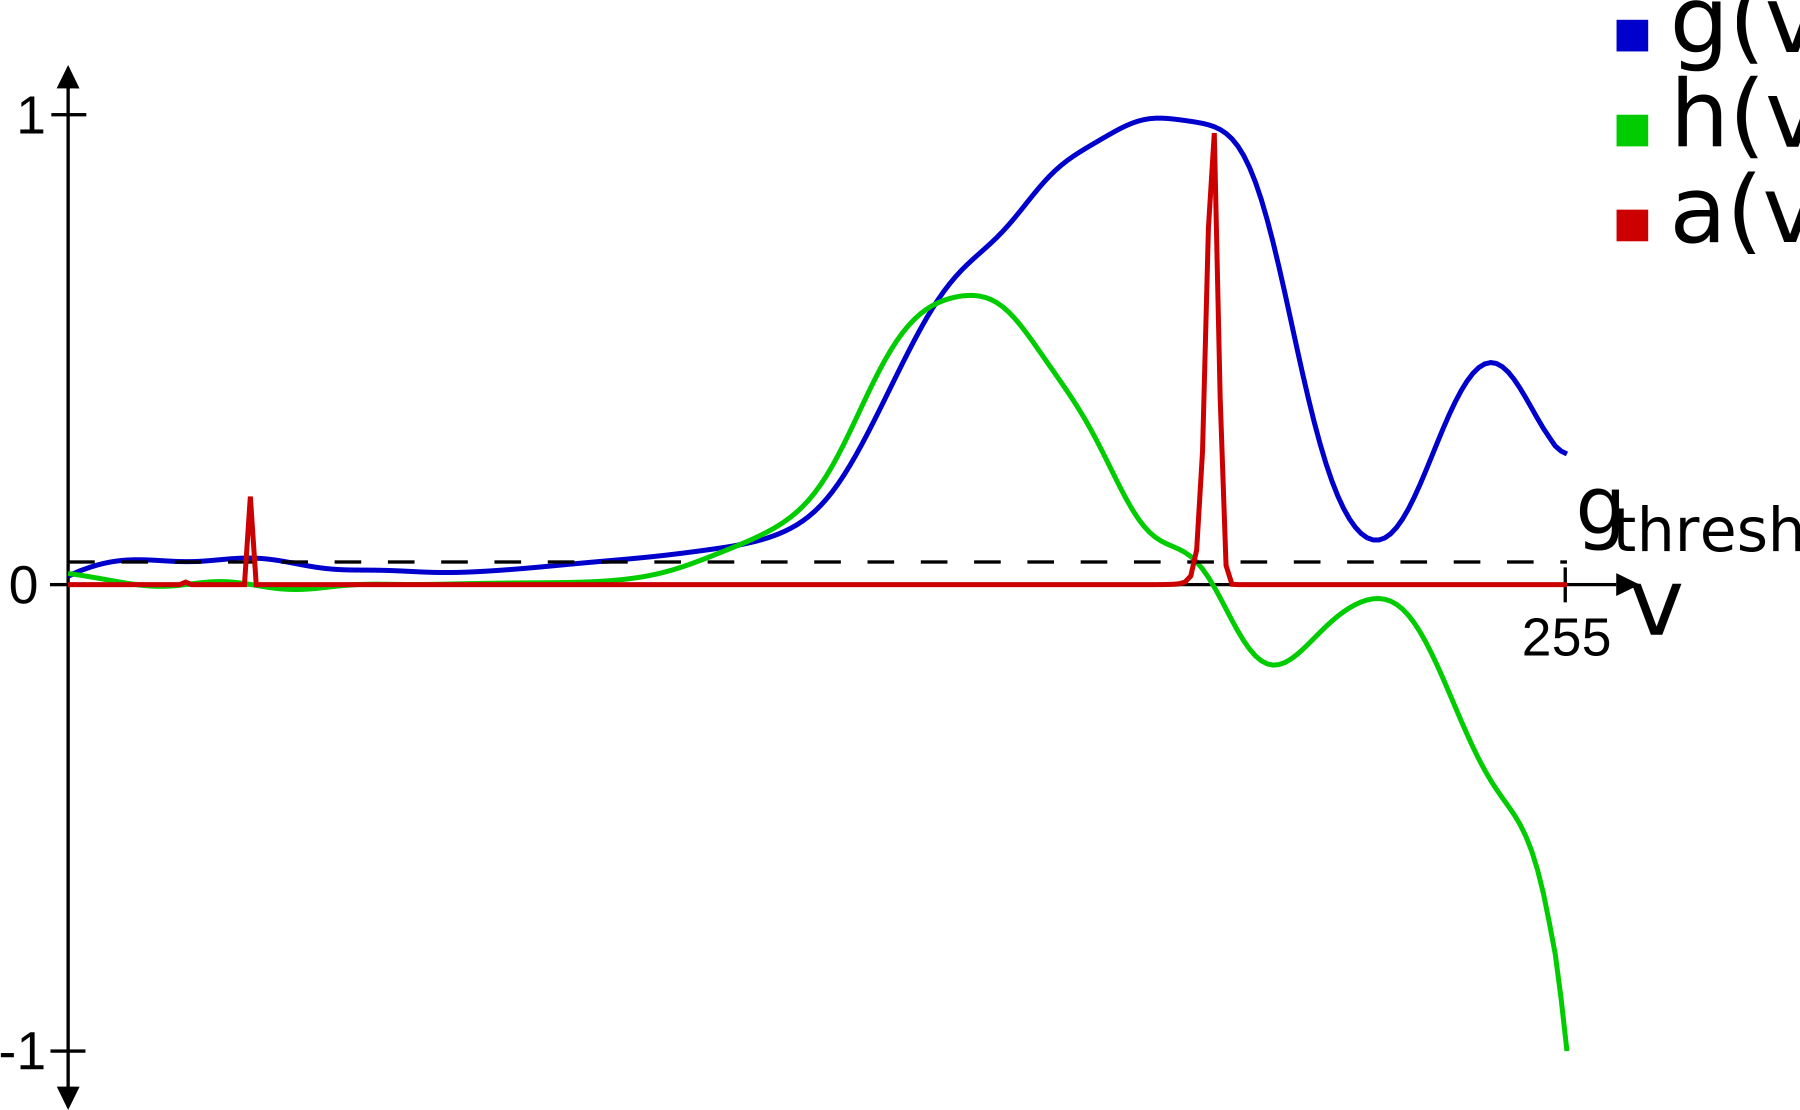
\includegraphics[width=0.65\textwidth]{images/r_vrep_so_kd_ft}
		\label{fig:r_vrep_kd}
	}
	\subfigure[Método proposto.]
	{
		\includegraphics[width=0.35\textwidth]{images/r_vrep_so_mine}
		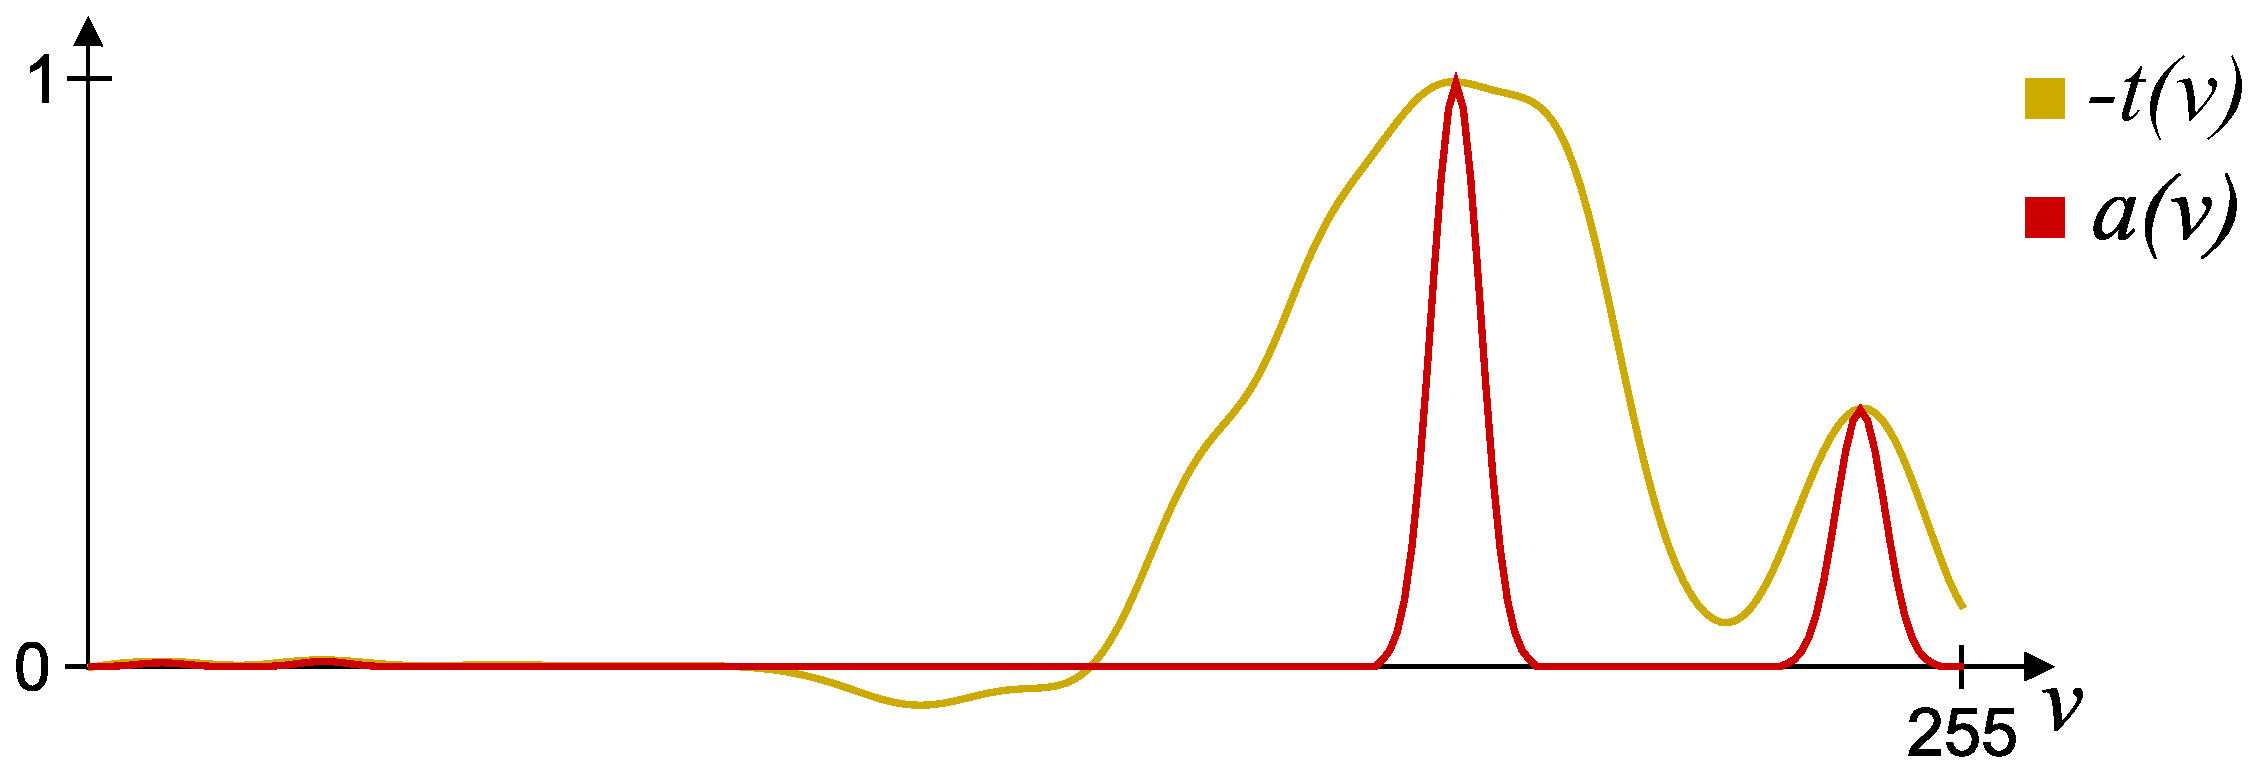
\includegraphics[width=0.65\textwidth]{images/r_vrep_so_mine_ft}			\label{fig:r_vrep_mine}
	}
	\caption{FT e visualização do volume de SO do modelo~A.}
	\label{fig:r_vrep}
\end{figure}

%%%%%%%%%%%%%%%%%%%%%%%%%%%%%%%%% VREP SO 2 %%%%%%%%%%%%%%%%%%%%%%%%%%%%%%%%%%%%
	A Figura~\ref{fig:r_vrep_2_slice} também exibe um volume de saturação de óleo (SO) do modelo~A, mas em outro momento da simulação. Este time step apresenta um caso mais difícil de se estimar o que deveria ser realçado como fronteira.
	
\begin{figure}[h]
	\centering
	\includegraphics[width=1\textwidth]{images/r_vrep_so_2_slice}
	\caption{Volume de saturação de óleo do modelo A.}
	\label{fig:r_vrep_2_slice}
\end{figure}

	A Figura~\ref{fig:r_vrep_2} mostra que os dois métodos detectaram uma fronteira em laranja. Esta isosuperfície condiz com a evolução da área invadida esperada para este modelo, como mostra a Figura~\ref{fig:r_reserv_livro}. Apesar das fronteiras excedentes não estarem mapeadas no avanço da área invadida, percebe-se que elas realçam interfaces entres diferentes regiões do reservatório. A relevância dessas fronteiras destacadas, no entanto, precisa ser avaliada com cautela e maior conhecimento sobre reservatórios.

\begin{figure}[h]
	\centering
	\subfigure[Método de \textit{Kindlmann e Durkin}.]
	{
		\includegraphics[width=0.35\textwidth]{images/r_vrep_so_2_kd}
		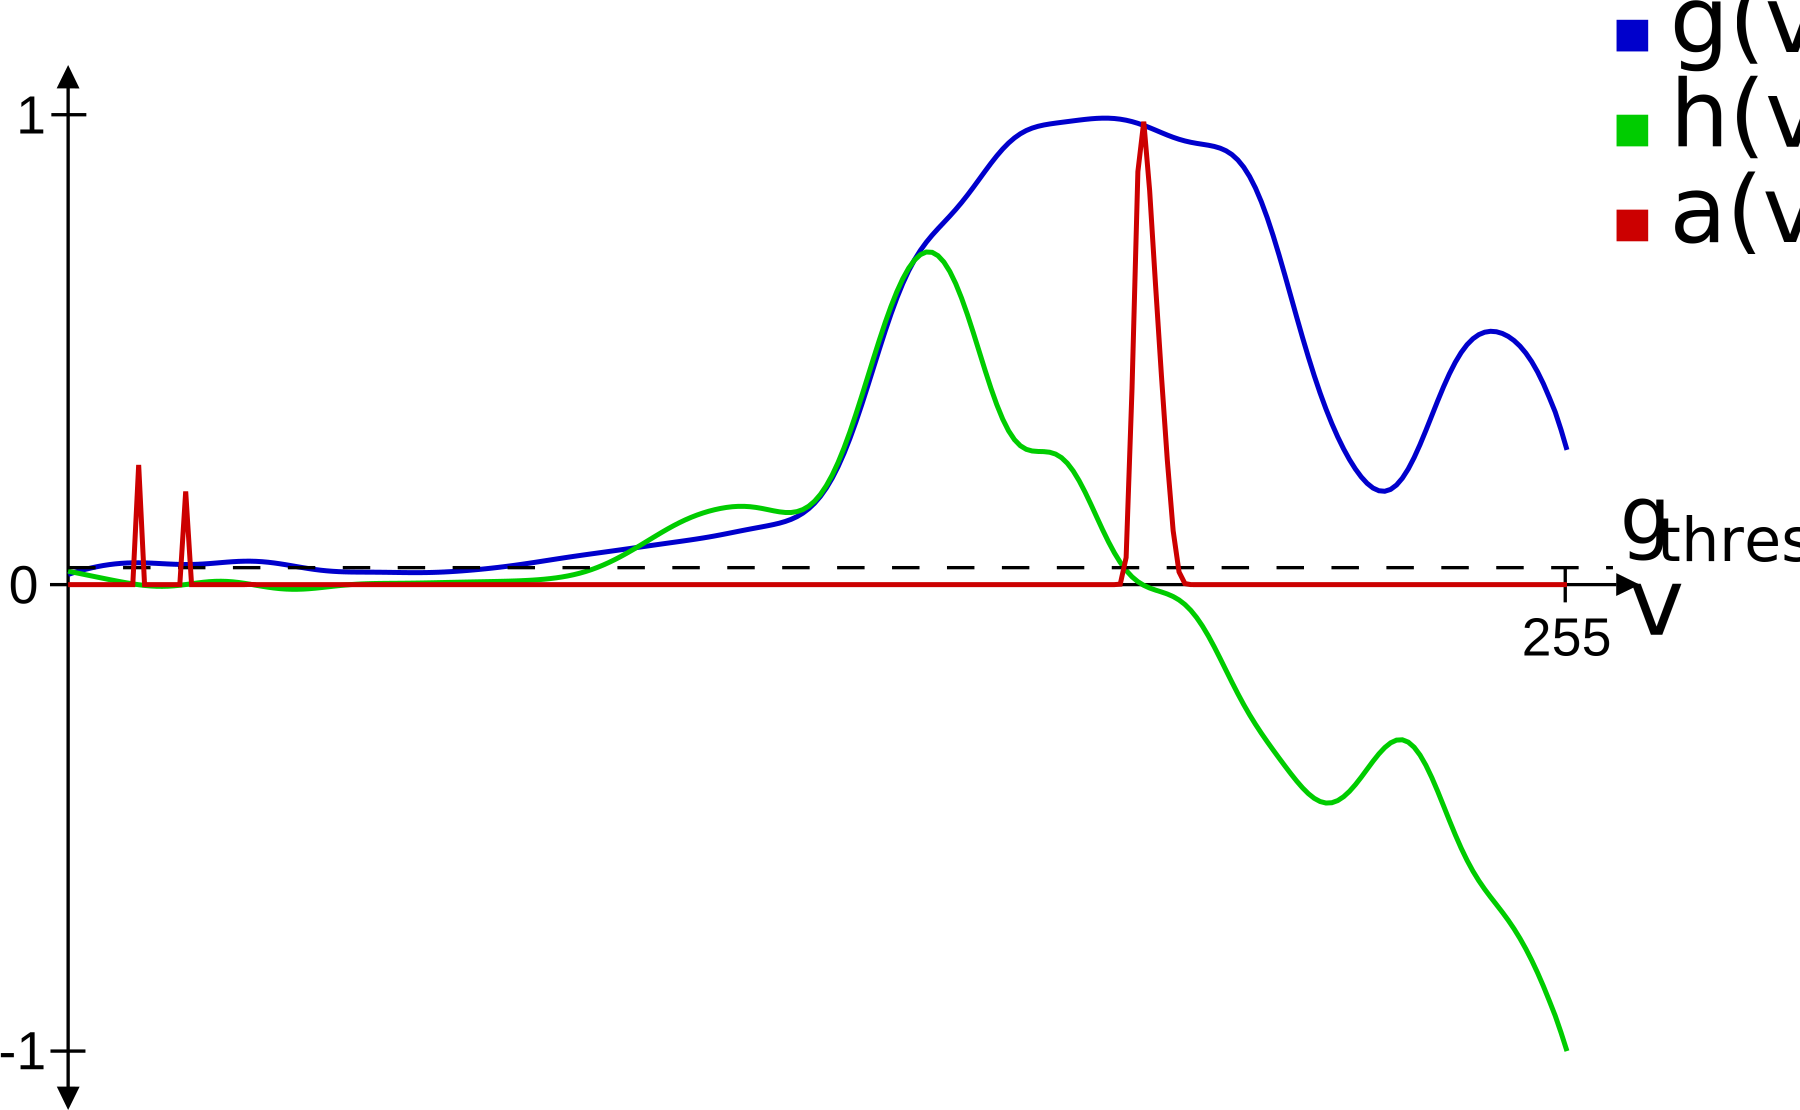
\includegraphics[width=0.65\textwidth]{images/r_vrep_so_2_kd_ft}
		\label{fig:r_vrep_2_kd}
	}
	\subfigure[Método proposto.]
	{
		\includegraphics[width=0.35\textwidth]{images/r_vrep_so_2_mine}
		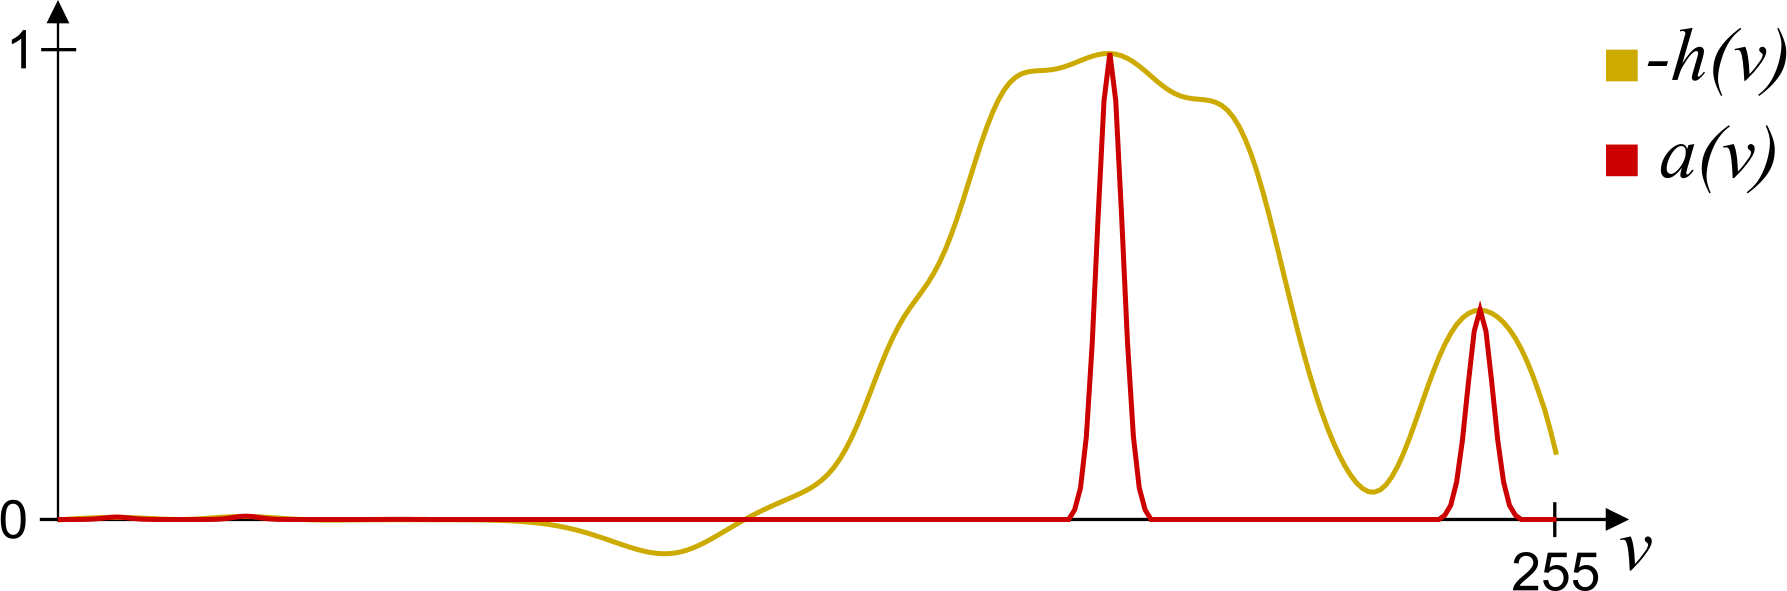
\includegraphics[width=0.65\textwidth]{images/r_vrep_so_2_mine_ft}			\label{fig:r_vrep_2_mine}
	}
	\caption{FT e visualização do volume de SO do modelo~A.}
	\label{fig:r_vrep_2}
\end{figure}

\begin{figure}[h]
	\centering
	\includegraphics[width=0.8\textwidth]{images/reserv_livro}
	\caption{Evolução da área invadida em uma malha de 5 pontos~\cite{rosa}.}
	\label{fig:r_reserv_livro}
\end{figure}
	
%%%%%%%%%%%%%%%%%%%%%%%%%%%%%%%%%% BOX SO %%%%%%%%%%%%%%%%%%%%%%%%%%%%%%%%%%%%%
	A Figura~\ref{fig:r_box_so_slice} mostra a simulação da saturação de óleo para o modelo de reservatório B. Comparando-a com as visualizações das Figuras~\ref{fig:r_box_so_kd}~e~\ref{fig:r_box_so_mine}, nota-se que as isosuperfícies realçadas pelos dois métodos, são interfaces entre regiões de SO distintas. Então, mais uma vez, cabe observar que as fronteiras destacadas pelo método de \textit{Kindlmann e Durkin} não correspondem aos pontos de maior primeira derivada.

\begin{figure}[h]
	\centering
	\includegraphics[width=0.95\textwidth]{images/r_box_so_slice}
	\caption{Volume de saturação de óleo do modelo B.}
	\label{fig:r_box_so_slice}
\end{figure}

\begin{figure}[h]
	\centering
	\subfigure[]
	{
		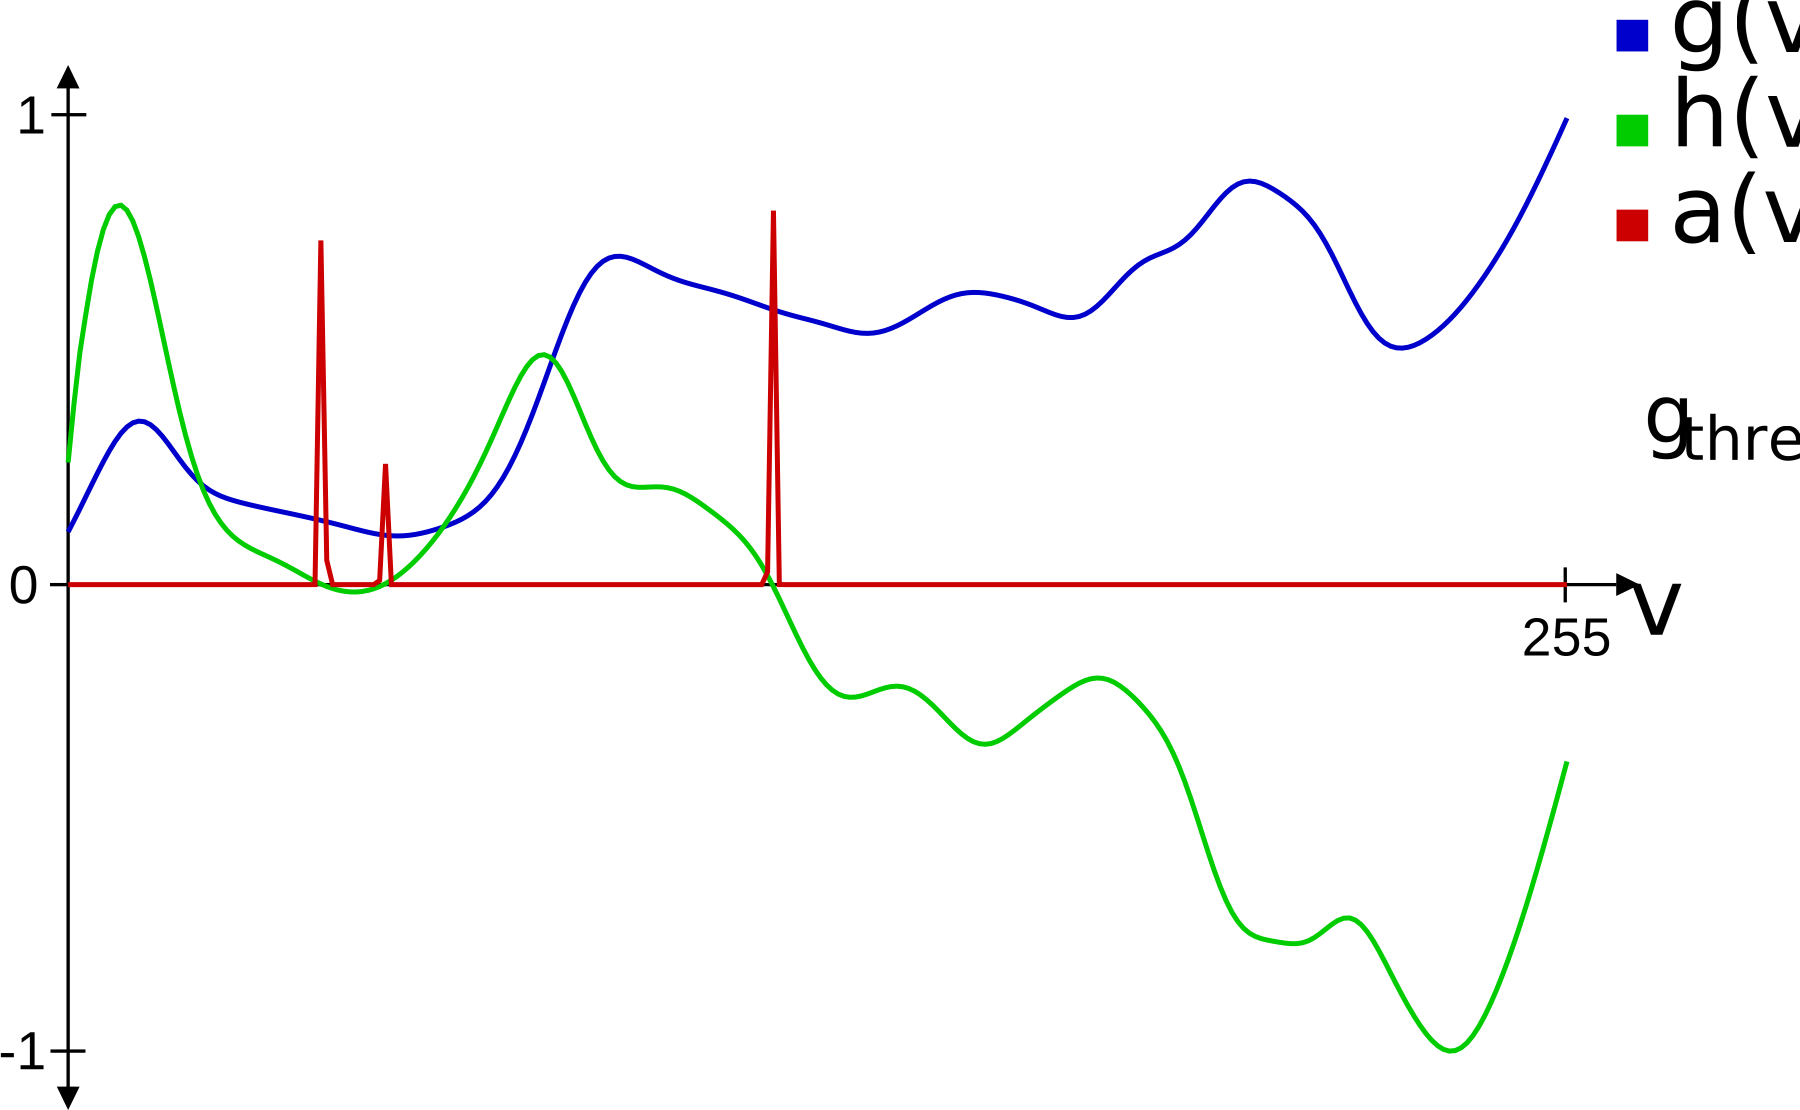
\includegraphics[width=0.7\textwidth]{images/r_box_so_kd_ft}
	}
	\subfigure[]
	{
		\includegraphics[width=0.7\textwidth]{images/r_box_so_kd}
	}
	\caption{FT e visualização do volume de SO do modelo~B pelo método de \textit{Kindlmann e Durkin}.}
	\label{fig:r_box_so_kd}
\end{figure}

\begin{figure}[h]
	\centering
	\subfigure[]
	{
		\includegraphics[width=0.7\textwidth]{images/r_box_so_mine_ft}
	}
	\subfigure[]
	{
		\includegraphics[width=0.7\textwidth]{images/r_box_so_mine}
	}
	\caption{FT e visualização do volume de SO do modelo~B pelo método proposto.}
	\label{fig:r_box_so_mine}
\end{figure}

%%%%%%%%%%%%%%%%%%%%%%%%%%%%%%%%%% BOX SG %%%%%%%%%%%%%%%%%%%%%%%%%%%%%%%%%%%%%
	A Figura~\ref{fig:r_box_sg_slice} mostra a simulação da saturação de gás (SG) para o modelo de reservatório B. O método de \textit{Kindlmann e Durkin} detecta apenas uma fronteira, como pode ser visto na Figura~\ref{fig:r_box_sg_kd}. Já o método proposto nesta dissertação, destava seis fronteiras. A menor delas realça a isosuperfície vermelha da Figura~\ref{fig:r_box_sg_kd}~\ref{fig:r_box_sg_kd_ft}, enquanto as outras realçam isosuperfícies paralelas e próximas àquela identificada pelo método de \textit{Kindlmann e Durkin}.
	
	Observando a Figura~\ref{fig:r_box_sg_slice}, fica claro que as isosuperfícies paralelas na Figura~\ref{fig:r_box_sg_mine} representam uma única fronteira de interesse no reservatório, entre as cores azul e laranja. Contudo, a última fronteira destacada pelo método proposto revela uma superfície de área invadida que não pode ser observada sem a aplicação de uma função de transferência.\\
	
\begin{figure}[h]
	\centering
	\includegraphics[width=1\textwidth]{images/r_box_sg_slice}
	\caption{Volume de saturação de gás do modelo B.}
	\label{fig:r_box_sg_slice}
\end{figure}

\begin{figure}[h]
	\centering
	\subfigure[]
	{
		\includegraphics[width=0.7\textwidth]{images/r_box_sg_kd_ft}
		\label{fig:r_box_sg_kd_ft}
	}
	\subfigure[]
	{
		\includegraphics[width=0.65\textwidth]{images/r_box_sg_kd}
	}
	\caption{FT e visualização do volume de SG do modelo~B pelo método de \textit{Kindlmann e Durkin}.}
	\label{fig:r_box_sg_kd}
\end{figure}

\begin{figure}[h]
	\centering
	\subfigure[]
	{
		\includegraphics[width=0.7\textwidth]{images/r_box_sg_mine_ft}
	}
	\subfigure[]
	{
		\includegraphics[width=0.7\textwidth]{images/r_box_sg_mine}
	}
	\caption{FT e visualização do volume de SG do modelo~B pelo método proposto.}
	\label{fig:r_box_sg_mine}
\end{figure}

%%%%%%%%%%%%%%%%%%%%%%%%%%%%%%%%%% BOX SW %%%%%%%%%%%%%%%%%%%%%%%%%%%%%%%%%%%%%
\clearpage
	A Figura~\ref{fig:r_box_sw_slice} mostra a simulação da saturação de água (SW) para o reservatório B. Esse modelo exemplifica bem a diferença entre os dois métodos quanto ao número de fronteiras, pois, assim como no modelo anterior, o método de \textit{Kindlmann e Durkin} detecta apenas uma fronteira, que pode ser vista na Figura~\ref{fig:r_box_sw_kd}. A detecção está correta e realça bem a fronteira entre o amarelo e o azul.
	
	No entanto, o método de \textit{Kindlmann e Durkin} não é capaz de realçar a fronteira existente entre as regiões vermelha e amarela. Observando a escala de cores, na Figura~\ref{fig:r_box_sw_slice}, vê-se que a fronteira não detectada possui mesma importância que a detectada, pois o range de valores que estas abrangem é similar. A fronteira faltante na detecção do método de \textit{Kindlmann e Durkin} é corretamente destacada pelo método proposto nesta dissertação. Na~Figura~\ref{fig:r_box_sw_mine} vê-se a isosuperfície esperada no formato de um cone vermelho. O método proposto destaca também a mesma fronteira encontrada por \textit{Kindlmann e Durkin}, além de quatro outras intermediárias.
	
	Por fim, é impostante observar que a fronteira ideal entre a região amarela e a azul, deveria destacar uma isosuperfície verde, dividindo todo o volume, uma vez que a escala de cores da função de transferência é a mesma do modelo. Porém os dois métodos tiveram deslocamento dessa fronteira.
	
\begin{figure}[h]
	\centering
	\includegraphics[width=1\textwidth]{images/r_box_sw_slice}
	\caption{Volume de saturação de água do modelo B.}
	\label{fig:r_box_sw_slice}
\end{figure}

\begin{figure}[h]
	\centering
	\subfigure[]
	{
		\includegraphics[width=0.7\textwidth]{images/r_box_sw_kd_ft}
		\label{fig:r_box_sw_kd_ft}
	}
	\subfigure[]
	{
		\includegraphics[width=0.7\textwidth]{images/r_box_sw_kd}
	}
	\caption{FT e visualização do volume de SW do modelo~B pelo método de \textit{Kindlmann e Durkin}.}
	\label{fig:r_box_sw_kd}
\end{figure}

\begin{figure}[h]
	\centering
	\subfigure[]
	{
		\includegraphics[width=0.7\textwidth]{images/r_box_sw_mine_ft}
	}
	\subfigure[]
	{
		\includegraphics[width=0.7\textwidth]{images/r_box_sw_mine}
	}
	\caption{FT e visualização do volume de SW do modelo~B pelo método proposto.}
	\label{fig:r_box_sw_mine}
\end{figure}

%%%%%%%%%%%%%%%%%%%%%%%%%%%%%%%%%% Pituba %%%%%%%%%%%%%%%%%%%%%%%%%%%%%%%%%%%%%
\clearpage
	A Figura~\ref{fig:r_pituba} mostra um momento da simulação da saturação de óleo de um modelo real de reservatório de petróleo, o Pituba. Essa visualização, feita pelo Geresim, incorpora uma função de transferência gerada automaticamente pelo método proposto nesta dissertação. Para este caso, não gerou-se uma função de opacidade mas uma função de peso, isto é, o valor da FT gerada multiplica cada coordenada rgb da FT de cores do Geresim. Assim, as fronteiras são realçadas através de cores mais claras, enquanto todo o resto do modelo possui tonalidades mais escuras.
	
\begin{figure}[h]
	\centering
	\includegraphics[width=1\textwidth]{images/pituba}
	\caption{Visualização do modelo Pituba através do Geresim, com uma FT gerada automaticamente pelo método descrito nesta dissertação.}
	\label{fig:r_pituba}
\end{figure}
	
	Nesta figura observa-se fronteiras (de cor laranja) circundando os poços de injeção (em azul). Essas regiões são consistentes com as fronteiras de avanço esperadas, já que é a partir dos poços de injeção de água que se formaram as interfaces entre a água e o óleo e, portanto, obtém a maior variação na saturação de óleo. Sendo assim, as fronteiras identificadas são bons indícios de onde se encontram as frentes de avanço.